\documentclass[12pt]{extarticle}
\usepackage[english]{babel}
\usepackage{NotesTeX}
\usepackage{subfigure}
\usepackage{tikz}
\usetikzlibrary{arrows}
\usepackage{multirow}
\usepackage{listings}
\usepackage{extarrows}
\usepackage{parskip}
\usepackage{eurosym}
\usepackage{footmisc}

\graphicspath{{../output/}}

\collaborationImg{
\includegraphics[width=30mm]{../../pictures/UIO.png}}

\author{\Large Håkon Olav Torvik, Vetle Vikenes \& Sigurd Sørlie Rustad}
\title{\Huge Machine Learning: Using regression and neural networks to fit continuous functions and classify data}
\affiliation{\large FYS-STK4155 – Applied Data Analysis and Machine Learning
\\Autumn 2021\\Department of Physics\\University of Oslo\\\\\today}
\begin{document}
\abstract{
	Abstract coming soon.
}
\maketitle
\pagestyle{myplain}
\section{Introduction}
In the modern world, digital data has become one of the most valuable commodities there is. Not because of scarcity, like most other valuables, but rather the exact opposite; the vast abundance of data available makes being able to understand trends and patterns in it extremely valuable for companies looking for profit. However, data is complex, having many features, and understanding how one affect another is impossible with purely human analysis. Luckily, there exists statistical methods that let us find the deeper connections, make models and even predict outcomes. In this paper we wish to study some stochastic methods, and look at their limitations and strengths.

First we will study a bi-variate continuous function known as the Franke function. We will use both stochastic gradient decent and a feed-forward deep neural network, with back propagation. Then we can also compare results with those obtained in a previous paper, using the deterministic methods ordinary least squares and ridge regression. Note that all methods used in this report is briefly covered in the theory section.

Next we will embark on a classification problem, using measurments of tumors in breast tissue to predict wether they are benign or malignant. Here we will again use a feed-forward deep neural network, along with logistic regression.

We will on no way answer all questions linked to the aforementioned methods. Such that anyone can reproduce or continue our studies, we list all the code, results and instructions on running the code in our GitHub repository\footnote{\href{https://github.com/sigurdru/FYS-STK4155/tree/main/project1}{https://github.com/sigurdru/FYS-STK4155/tree/main/project2}}.

\section{Theory}
In the theory-section we aim to give a brief explanation of the main concepts and terminology used in this report. For a more in-depth explanation we recommend reading the appropriate sections in \cite{2019}, which has been of great inspiration and help for us throughout the project.

In general, we have a dataset $\bo x$, where each point $\bo x_i$ takes a value $y_i$, for which we want to make a model $\bbeta$, such that for a new data point $\bo x_k \notin \bo x$ we can make a prediction for the value $y_k$.  The model $\bbeta$ is a vector, where each element is a parameter of our model, such that $\bbeta$ is sometimes called the parameters. For gradient decent, we have to chose what shape the model should be, as was done for linear regression in \cite{project1}, while the neural network makes its own model.

\subsection{Gradient Decent}\label{sec:GD}
In this section we cover gradient decent and different variations of it. More specifically we describe gradient decent (GD), stochastic gradient decent (SGD) and adding momentum to the aforementioned methods. All gradient decent methods start with an initial guess for what the model $\bbeta$ should be, and iteratively updates the guess by training on the dataset, either until it reaches a minimum, or a certain number of iterations have been performed.
\subsubsection{Ordinary Gradient Decent}
Gradient decent methods is often used to minimize the so-called cost/loss-function, which tells us how good our model at predicting the dataset is (more on this in section \ref{sec:cost_func_and_regul}). For now, we use a general cost function $C(\bbeta)$ for a given model $\bbeta$, which can be expressed as the sum over the cost function for each datapoint $\bo x_i$, as such:
\begin{equation}
	C(\boldsymbol{\beta}) = \sum_{i = 1}^{n}c_i(\mathbf{x}_i, \boldsymbol{\beta}),
\end{equation}
where $n$ denotes the number of datapoints. The gradient with respect to the parameters $\bbeta$, which represent the direction of optimal minimization of the cost function,  is then defined as
\begin{align}
	\nabla_{\boldsymbol{\beta}} C(\boldsymbol{\beta}) = \sum_{i = 1}^{n} \nabla_{\boldsymbol{\beta}} c(\mathbf{x}_i, \boldsymbol{\beta}).
	\label{eq:Total_gradient}
\end{align}
The algorithm for GD is then:
\begin{align}
	\mathbf{v}_t             & = \eta \nabla_{\boldsymbol{\beta}} C(\boldsymbol{\beta}_t) \nonumber \\
	\boldsymbol{\beta}_{t+1} & = \boldsymbol{\beta}_t - \mathbf{v}_t,
	\label{eq:GD_algo}
\end{align}
where $\eta$ is what we call the learning rate, representing the step-length to move in the optimal direction.  This algorithms iteratively finds a new $\boldsymbol{\beta}_{t+1}$ which (ideally) decreases the cost function. This is of course not always the case, and depends on the value of $\eta$.

For a model with $p$ parameters, the cost-function is the surface of a $p$-dimensional hypersurface, and minimizing this can lead to several problems. For example, if $\eta$  is too big, the cost-function can diverge and never find a minimum of the hypersurface, while if $\eta$ is too small we will need too many iterations to reach a minimum in reasonable time. One method of avoiding the cost-function diverging, is using a dynamic learning schedule, where the learning rate $\eta$ decreases during training. Our model then makes larger steps in the beginning, and then smaller and smaller, such that we should be able to converge to a minimum, and not making too big steps, circling around it.

An additional problem is that the  hypersurface is not a smooth terrain with a single minimum. Our model can potentially move down into a local minimum, which can be close to the level of the global minimum, or far worse than it. When our model converges, we have no way of knowing if we have found the optimal, global minium, or are stuck in one of the many local minima, with no way of getting out.


\subsubsection{Stochastic Gradient Decent}\label{sec:SGD}
With large datasets, a large number of computations is needed when calculating the gradient. It takes a lot of time, and the model is only updated once per iteration, making improvement slow. Stochastic Gradient Decent. SGD, combats this by approximating the total gradient \eqref{eq:Total_gradient}. This is done by performing  gradient decent on a subset of the data, called a minibatch. With $n$ still denoting the total number of datapoints, we will have $N_B=n/M$ minibatches, where $M$ is the size of each minibatch. The minibatches are denoted by $B_k$. Thus our approximated gradient for a single minibatch $B_k$ is defined as
\begin{align}
	\nabla_{\boldsymbol{\beta}} C^{MB}(\boldsymbol{\beta}) \equiv \sum_{i \in B_k}^M \nabla_{\boldsymbol{\beta}} c(\mathbf{x}_i, \boldsymbol{\beta}).
\end{align}
Then the aim is to use this approximated gradient, for all $N_B$ minibatches, to update the parameters $\boldsymbol{\beta}$, at every step $k$. Doing this for all $N_B$ minibatches, are what we refer to as an epoch. The SGD algorithm then becomes very similar to \eqref{eq:GD_algo}, however with an approximated gradient.
\begin{align}
	\mathbf{v}_t             & = \eta\nabla_{\boldsymbol{\beta}} C^{MB}(\boldsymbol{\beta}_t) \nonumber \\
	\boldsymbol{\beta}_{t+1} & = \boldsymbol{\beta}_t - \mathbf{v}_t
	\label{eq:SGD_algo}
\end{align}
Choosing a smaller $M$ gives a worse approximation of the full gradient, though at the same time the model will have more chances to move in the correct direction. Further, by choosing $M$ such that $N_B$ is neither too small or large, our program will run faster. This not only speeds up our program, it also helps prevent getting stuck in local minima because of the stochastic nature. The dataset is shuffled after each epoch, creating new minibatches such that we never use the same one twice.

\subsubsection{Adding Momentum}
These methods can still be optimized further by adding momentum. This is done by adding a term to the parameter $\mathbf{v}_t$ in equations \eqref{eq:GD_algo} and \eqref{eq:SGD_algo}. This so-called mass term, simulates the gradient having momentum, such that every update of $\bbeta$ is a running average.
\begin{align} \label{eq:vt_mom}
	\mathbf{v}_t = \eta \nabla_{\boldsymbol{\beta}_t} C(\boldsymbol{\beta}) \rightarrow \mathbf{v}_t = \gamma \mathbf{v}_{t-1} + \eta \nabla_{\boldsymbol{\beta}} C(\boldsymbol{\beta}_t).
\end{align}
Here $\gamma \in [0, 1]$ is what we could refer to as the mass, and is a free parameter. One of the benefits is for example that this lets us move faster in regions where the gradient is small.

\subsection{Logistic Regression}\label{sec:logistic_regression}
Gradient decent is used when we have a continuous output, like fitting a function to data. Logistic Regression is used for classification problems, meaning that we want to predict discrete outputs, for instance true or false, given a set of information about a subject. This is the case for binary classification, where we only have one output. It is also possible to use multi-class classification, where one has several outputs, each representing the probability of the class being given by that output.\sn{kanskje flytt denne setningen til senere?} In our case we want a model that takes in some values $\mathbf{x}_i$ and spits out zero or one. These values should correspond to the actual classification $y_i\in\{0,1\}$ corresponding to true or false respectively. Lets define our model as
\begin{align}
	\sigma(s_i), \ \ \text{where }s_i = \bo x_i^T \bo w + b_0 \equiv \bo X_i^T \bo W,
	\label{eq:log_reg_model}
\end{align}
where $\bo x_i^T$ is our inputdata, $\bo w$ and $b_0$ are parameters in the model. As a shorthand we also defined $\bo W = (b_0, \bo w)$ and $\bo X_i = (1, \bo x_i)$. We also have $\sigma$ which is some soft classifier that maps our output between zero and one (i.e. the Sigmoid \eqref{eq:sigmoid}). The reason why we want a soft classifier and not a hard one (like $\sigma = 1$ if $s\geq0$ and $0$ otherwise), is because then we can interpret the output as a probability, quantifying how certain the model is in its prediction. Here we also need a cost function to minimize. It is common to choose the cross entropy, which we derive in \ref{sec:cost_func_and_regul}. However we will just use it without derivation for now. The cross entropy for this model is given as
\begin{align}
	C(\bo W) = \sum_{i = 1}^{n} -y_i \log\sigma(\bo X_i^T \bo W) - (1 - y_i)\log\left[1 - \sigma(\bo X^T_i \bo W)\right],
	\label{eq:cross_entropy2}
\end{align}
where $n$ are the number of samples we want to classify, and $y_i$ the true classification. Now with a cost function and model in hand we are ready to minimize the cost function in order to find the optimal parameters for the model. We have a convex cost function, therefore a minimization leads to
\begin{align}
	\nabla_{\bo W} C(\bo W) = \sum_{i = 1}^n \left[\sigma(\bo X_i^T \bo W - y_i)\right]\bo X_i.
	\label{eq:cross_entropy_grad}
\end{align}
Thus the only thing left to do is perform an algorithm similar to \ref{eq:SGD_algo}, where the parameters to update are $\bo W$.

\subsection{Feed-Forward Deep Neural Networks}\label{sec:NeuralNetwork}
Neural networks are neural-inspired nonlinear models, which are taught by a way of learning. We will in this section explain what we mean by non-linearity, the basic architecture of a neural network and how the network learns. In this paper, only supervised learning will be studied, where we train our model on fully labeled data, as opposed to unsupervised learning, where the model first is shown unlabeled data.

\subsubsection{Architecture of Neural Networks}
The structure we are going to use in this report is similar to that in figure \ref{fig:neural_network}. The gray circles are what we refer to as nodes. For now we just need to know that they hold some numerical value. One initializes the network by giving the nodes in the input layer numerical values. These values would correspond to some actual physical property, for example brightness of pixels in a picture. Then, each node in the input layer is connected to each node in the hidden layer $h_1$. In figure \ref{fig:neural_network} we have three such hidden layers, where each node in one layer is connected to every node in the next layer. Now the nodes are connected through what we will refer to as weights, biases and activation functions (more on that later). The connections are what assigns the numerical value of the nodes in the next layer. Lastly we have the output layer, which outputs values dependent on the problem. If we have a classification situation, where we for example wanted to classify the type of animal in different pictures, then one node could correspond to  a lion, next to a zebra and so fourth. By this we would know what animal the network \textit{thinks} is in the picture by looking at what neuron has the highest numerical value.

The structure for the neural net we use in this report is similar to that in figure \ref{fig:neural_network}. The gray circles are what we refer to as nodes, organized into layers. They hold some numerical value. The first and last layer are the input and output layer, respectively. The rest are called hidden layers, denoted $h_i$. In figure \ref{fig:neural_network} three hidden layers are shown. Between each layer is a set of weights, connecting each node in the preceding layer to each node in the succeding one. One initializes the network by giving the nodes in the input layer numerical values. These values would correspond to some actual physical property, for example brightness of pixels in a picture. Then, the values are fed forward, the values of the nodes in the next layer being the weighted sum of the values in the previous, plus a bias $b$. The values are \textit{activated} by an activation function, before similarly being fed forward to the next layer, until reaching the output layer. The the case of regression, the output layer is a single node, giving the functional value. In the case of classification, for example classifying the type of animal in pictures, one node could correspond to a lion, next to a zebra and so fourth. By this we would know what animal the network predicts is pictured by finding the neuron has the highest numerical value.

\begin{figure}[h]
	\minipage{0.70\textwidth}
	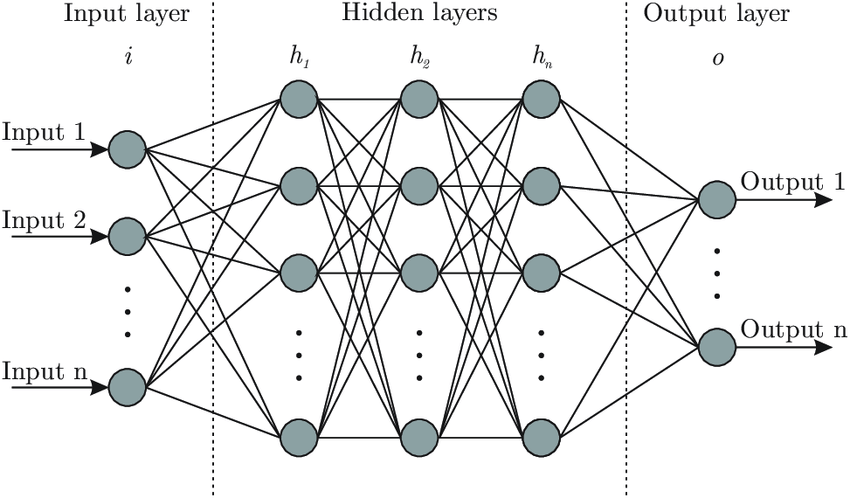
\includegraphics[width=\linewidth]{pictures/neural_network.png}
	(source: \texttt{https://www.researchgate.net/figure/Artificial-neur
		al-network-architecture-ANN-i-h-1-h-2-h-n-o\_fig1\_321259051})
	\endminipage\hfill
	\minipage{0.29\textwidth}
	\caption{Basic outline of a neural network. It displays the different layers (input, hidden and output), nodes (gray circles) and the connection between the nodes (black lines).}\label{fig:neural_network}
	\endminipage
\end{figure}

We mentioned that the different nodes are connected through weights, biases and activation functions. Looking at figure \ref{fig:neural_network}, a neuron $j$ in layer $h_1$ is connected to $n$ input neurons, denoted by black lines. Each input neuron has a numerical value defined by the problem. The value neuron $j$ in $h_1$ then gets is defined as
\begin{align}
	a_{h_1, j} = \sigma (x_1w_1 + x_2w_2 + \dots + x_nw_n + b_j),
\end{align}
where $x_i$ are the values of neuron $i$ in the input layer, $w_i$ are the weights between neurons $i$ and $j$, $b$ is what we refer to as the bias and $\sigma$ is the activation function. Every neuron is connected like this, with different weights and biases. Initially the network will make random predictions. Through training, the weights and biases are updated using the backpropagation algorithm, described in section \ref{sec:back_prop}, until the predictions become extremely accurate.

\subsubsection{Activation Functions}
The activation functions are where the non-linearity of the neural nets comes in, because they are non-linear. Now there are many such functions, in our project we have implemented the 3 displayed in figure \ref{fig:activation_functions}. The exact functions are as follows
\begin{align}
	\text{Sigmoid: }\sigma(x)    & = \frac{1}{1 + e^{-x}},\label{eq:sigmoid}          \\
	\text{RELU: }\sigma(x)       & = \max(0,x), \label{eq:RELU}                       \\
	\text{Leaky RELU: }\sigma(x) & = \begin{cases}
		\alpha x, & \text{if } x\leq 0 \\
		x,        & \text{otherwise}.
	\end{cases} \label{eq:leaky_RELU}
\end{align}
For Leaky RELU, $\alpha$ is some parameter for which we set to $\alpha = 0.01$.

\begin{figure}[h]
	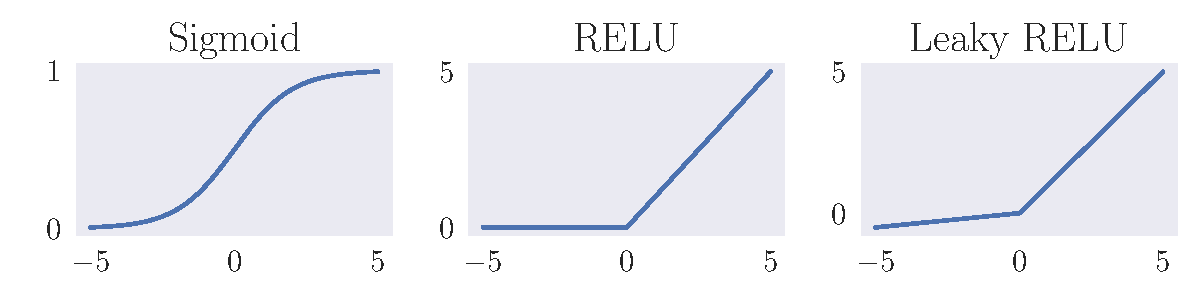
\includegraphics[width=\linewidth]{pictures/activation_functions.pdf}
	\caption{Some activation functions, Sigmoid, RELU and Leaky RELU, respectively.}\label{fig:activation_functions}
\end{figure}

All neurons in all hidden layers are activated by the same activation function. The input layer is just the input, so it is not activated. In the case of regression, then the output layer is not activated. Then the predicted function value is just the weighted sum from the last hidden layer. In the case of classification, we want the values in the output nodes to indicate probabilities. Thus, we use an activation function that considers the value in the other nodes in the other output nodes. The softmax function does this.

\begin{equation*}
	\sigma(z_i) = \frac{e^{z_i}}{\sum_{j=1}^Ke^{z_j}},
\end{equation*}
where $K$ is the number of classes, output nodes.

\subsubsection{Cost Function and Regularization}\label{sec:cost_func_and_regul}
Before one can start training the data, we must have a cost function. This will quantify how well or poorly our network is performing, and is what we want to minimize when we train the network. For continuous data it is common to use mean square error (MSE) as the cost function. It is just the difference between desired output ($\hat{\mathbf{x}}$) and actual output ($\mathbf{x}$), squared, averaged over all datapoints $\bo x_i$, as such
\begin{align}
	C(\mathbf{x}) = \frac{1}{n}\sum_{i=1}^{n}(\hat{\mathbf{x}}_i - \mathbf{x}_i)^2.
	\label{eq:MSE}
\end{align}

As was done with linear regrssion, \cite{project1} regularization can help prevent overfitting. Common regularization methods are $L_1$ and $L_2$ penalties, which add a regularization term to the cost function, as such
\begin{align}
	L_1: \ \ C(\mathbf{x}) & = \frac{1}{n}\sum_{i=1}^{n}(\hat{\mathbf{x}}_i - \mathbf{x}_i)^2 + \lambda\sum_j \abs{\mathbf{W}_j}, \label{eq:L1} \\
	L_2: \ \ C(\mathbf{x}) & = \frac{1}{n}\sum_{i=1}^{n}(\hat{\mathbf{x}}_i - \mathbf{x}_i)^2 + \lambda\sum_j \mathbf{W}^2_j, \label{eq:L2}
\end{align}
where $\lambda$ is some regularization parameter and $\mathbf{W}$ are the weights and biases. We will in this paper study the effects of adding a $L_2$-regulizer term when updating the parameters, by adding the term $\eta \lambda \mathbf{W}_{t-1}$ to equation \eqref{eq:vt_mom}.

We mentioned when talking about logistic regression (section \ref{sec:logistic_regression}), that for classification scenarios one will often use cross-entropy as the cost function. Continuing with the model defined by \eqref{eq:log_reg_model}, we want to find an appropriate cost function. We define the probability of an outcome $y_i$ given parameters $\bo X_i$ and $\bo W$ as
\begin{align}
	P(y_i = 1|\bo X_i, \bo W) & = \frac{1}{1 + \exp(-\bo X_i^T \bo W)}, \\
	P(y_i = 0|\bo X_i, \bo W) & = 1 - P(y_i = 1|\bo X_i, \bo W)
\end{align}
We can then map these probabilities to our soft classifier $\sigma(s_i)$
\begin{align}
	P(y_i = 1) = \sigma(s_i) = \sigma(\bo X_i^T \bo W).
\end{align}
Now we can define the cost function using Maximum Likelihood Estimation (MLE), which states that we should choose parameters that maximize the probability of our given data. Consider the dataset $\mathcal{D}\{(y_i, \bo x_i)\}$, where we remind that $\bo x_i$ are the input parameters. Then the probability of our dataset given $\bo W$ is
\begin{align}
	P(\mathcal{D}|\bo W) = \prod_{i=1}^{n} \left[\sigma(\bo X_i^T\bo W)\right]^{y_i} \left[1 - \sigma(\bo X_i^T\bo W)\right]^{(1 - y_i)}.
\end{align}
Again we remind that $n$ are the number datapoints we want to classify. This expression is difficult to work with, thus we take the logarithm.
\begin{align}
	l(\bo W) = \log(P(\mathcal{D}|\bo W)) = \sum_{i = 1}^n y_i\log(\sigma(\bo X_i^T \bo W)) + (1-y_i)\log(1 - \sigma(\bo X_i^T \bo W))
\end{align}
MLE entails finding the $\bo W$ that maximizes $l(\bo W)$, or more commonly, minimizes $-l(\bo W)$. Thus our cost function becomes
\begin{align}
	C(\bo W) = -l(\bo W) = \sum_{i = 1}^{n} -y_i \log\sigma(\bo X_i^T \bo W) - (1 - y_i)\log\left[1 - \sigma(\bo X^T_i \bo W)\right],
	\label{eq:cross_entropy}
\end{align}
which is equation \eqref{eq:cross_entropy2}.

\subsubsection{The Backpropagation Algorithm} \label{sec:back_prop}
With a desired cost function we are ready to train the neural network. This is done by the backpropagation algorithm. The method entails finding the derivative of the cost function, with respect to all parameters. When we have a neural network, we have thousands of parameters which can be tuned (weights and biases), meaning that we have to approximate the derivative somehow. The backpropagation algorithm does just that, by exploiting the layered structure displayed in figure \ref{fig:neural_network}.

Before we can embark on deriving the algorithm we will introduce some notation. We assume $L$ total layers, indexed as $l = 1, \dots , L$. Next we need to index the weights, nodes and biases. Let $w_{jk}^l$ be the weight connecting $k$-th neuron in layer $l-1$ and $j$-th neuron in layer $l$. The index order in $j$ and $k$ are such that we can do matrix multiplication with index notation later down the road. Further let $b_j^l$ be the bias for the $j$-th neuron in layer $l$. Thus the activation of the $j$-th neuron in layer $l$ ($a^l_j$) becomes
\begin{align}
	a_j^l = \sigma\left(\sum_{k} w_{jk}^l a_k^{l-1} + b_j^l\right) = \sigma(z_j^l), \ \ z_j^l \equiv \sum_{k} w_{jk}^l a_k^{l-1} + b_j^l.
	\label{eq:activation_of_node_ajl}
\end{align}
Here $\sigma$ is an activation function.

Now the cost function will depend directly on the activation of the output layer ($a^L_j$). However the activation of the output layer depends on the previous layers, meaning that the cost function depends indirectly on all the previous layers. Lets define define the error $\Delta_j^L$ of the $j$-th neuron in layer $L$, as the change in cost function with respect to $z^L_j$.
\begin{align}
	\Delta_j^L \equiv \del{C}{z_j^L}
	\label{eq:backprop0}
\end{align}
We can similarly define the error of neuron $j$ in layer $l$, as the change in the cost function with respect to $z_j^l$,
\begin{align}
	\Delta_j^l \equiv \del{C}{z_j^l} = \del{C}{a_j^l}\del{a_j^l}{z^l_j} = \del{C}{a_j^l}\der{\sigma(z^l_j)}{z^l_j}.
	\label{eq:backprop1}
\end{align}
In the next few lines we are going to derive several equations needed for the algorithm, it will be apparent why after we have found them. Notice that \eqref{eq:backprop1} also can be written as
\begin{align}
	\Delta_j^l = \del{C}{z_j^l} = \del{C}{b_j^l}\del{b_j^l}{z^l_j} = \del{C}{b_j^l}.
	\label{eq:backprop2}
\end{align}
Because $\partial b_j^l/\partial z^l_j = 1$ from \eqref{eq:activation_of_node_ajl}. Again using the chain rule we can rewrite \eqref{eq:backprop1}
\begin{align}
	\Delta_j^l & = \del{C}{z_j^l} = \sum_{k} \del{E}{z_k^{l+1}}\del{z_k^{l+1}}{z^l_j} = \sum_{k} \Delta_k^{l+1}\del{z_k^{l+1}}{z^l_j} \nonumber \\
	           & = \left(\sum_{k} \Delta_k^{l+1} w_{kj}^{l+1}\right)\der{\sigma(z^l_j)}{z^l_j}.
	\label{eq:backprop3}
\end{align}
To find the last equation, we differentiate the cost function with respect to the weight $w^l_{jk}$
\begin{align}
	\del{C}{w_{jk}^l} = \del{C}{z_j^l}\del{z_j^l}{w_{jk}^j} = \Delta l a_k^{l-1}.
	\label{eq:backprop4}
\end{align}
Now why have we done all this work, well because the equations \eqref{eq:backprop1}, \eqref{eq:backprop2}, \eqref{eq:backprop3} and \eqref{eq:backprop4} define what we call the backpropagation algorithm. Then, what exactly is the algorithm? In entails six steps:
\begin{description}
	\item[1 Activation:] First activate the neurons in the activation layer ($a^1_j$) with desired data.
	\item[2 Feedforward:] Activate the nodes in following layers, this is done by equation \eqref{eq:activation_of_node_ajl}.
	\item[3 Error at layer $L$:] Calculate the error at the last layer using \eqref{eq:backprop1}.
	\item[4 Backpropagate error:] With \eqref{eq:backprop3} we can the calculate the error, iterating backwards in the network.
	\item[5 Calculate gradient:] Find the gradient by using equations \eqref{eq:backprop2} and \eqref{eq:backprop4}.
	\item[6 Update parameters:] Update the parameters similarly to \eqref{eq:SGD_algo}, however $\boldsymbol{\beta}_t$ are our weights and biases in this case.
\end{description}

The expression for updating the weights and biases are
\begin{align}
	w_{jk}^l \leftarrow & w_{jk}^l - \eta \Delta_j^l a_k^{l-1} \label{eq:update_weights} \\
	b_j^l \leftarrow    & b_j^l - \eta \Delta_j^l \label{eq:update_biases}
\end{align}

\subsubsection{Initialization of weights}
We mentioned earlier than then the network is created, it has weights and biases between the layers. These needs to be initialized in some way. The biases are simple to initialize, as they are a single number for every node. These are initialized as a small, non-zero value $b_0$, which we choose as $b_0=0.01$.

Before 2006, most neural networks were performing quite badly on most tasks, as they did not learn during training. One of the (several) reasons were due to bad initialization of weights. A common way of doing this was using the standard normal distribution $W_{i,j} \sim  \mathcal{N}(0, 1)$. The problem with this is that it does not consider the size of the layers. In 2010, it was shown that when using sigmoid as the activation function, Xavier-initialization give better results \cite{xavier}. This is given as $W_{i, j}\sim\mathcal{U} \left(-\frac{1}{\sqrt{n}}, \frac{1}{\sqrt{n}} \right)$, where $\mathcal{U}$ is the uniform distribution, and $n$ is the number of nodes in the preceding layer.

In 2015, He-initialization was shown to work well with ReLU and Leaky ReLU \cite{He}. Here, the weights are initialized using the normal distribution, but with a variance given by $v = 2/(1 + \alpha^2)n$, where again $n$ is the number of nodes in the preceding layer, and $\alpha$ is the parameter of the Leaky ReLU-function. For ReLU, this is 0. These initializations only consideres the number of nodes in the preceding layer, though normalized initializations considering also the the number of nodes in the succeding layer could yeild better results. We use the initializations as given here, for the given activation-function, and will not study the particular effects of this in depth.



\section{Methods}
As we mentioned in the introduction, we wish to study different ways of fitting two types of datasets. The first which we can classify as \textit{continuous} is the Franke Function \eqref{eq:FF},
\begin{align}
	\begin{split}\label{eq:FF}
		f(x,y) = &\frac{3}{4}\exp(-\frac{(9x -2)^2}{4} - \frac{(9y-2)^2}{4}) + \frac{3}{4}\exp(-\frac{(9x + 1)^2}{49} - \frac{(9y + 1)}{10})
		\\
		+ &\frac{1}{2}\exp(-\frac{(9x-7)^2}{4} - \frac{(9y -3)}{4}) - \frac{1}{5}\exp(-(9x-4)^2 - (9y-7)^2).
	\end{split}
\end{align}
We will use both stochastic gradient decent and feed forward neural network to try and fit the data. Both methods are covered in the theory sections \ref{sec:GD} and \ref{sec:NeuralNetwork} respectively.

Next we will embark on an classification problem. Namely classifying if breast tissue is malignant or benign, by studying the data provided by Wisconsin breast cancer data\footnote{\href{https://www.kaggle.com/uciml/breast-cancer-wisconsin-data}{https://www.kaggle.com/uciml/breast-cancer-wisconsin-data}}. We will again use a feed forward neural network, and logistic regression. The latter is covered in the theory section \ref{sec:logistic_regression}.

\subsection{Franke Function}
In \cite{project1}, we already studied the Franke function using linear regression, specifically OLS and OLS with an L2 and L1 parameter $\lambda$, so-called Ridge and Lasso regression. The results from these methods will form the basis for comparing our results using SGD and neural networks. The rapport, along with the code can be found at our GitHub\footnote{\href{https://github.com/sigurdru/FYS-STK4155/tree/main/project1}{https://github.com/sigurdru/FYS-STK4155/tree/main/project1}}. In order to have comparable results, we will use the same parameters for the data. Only the methods will be different. In that project we generated the data using $N=30\times30$ uniformly distributed datapoints in $x$- and $y$-direction, respectively. To simulate it being real data, we also added normally distributed noise with mean zero and standard deviation $0.2$: $\epsilon \sim \mathcal{N}(0,0.2)$. We also split the input and target data in the same way as before, using $80\,\%$ of the data for training and $20\,\%$ of the data for testing. The two splitted data sets are then scaled by subtracting the mean of the relevant training data.

\subsubsection{Stochastic Gradient Descent}
As in \cite{project1}, we have to choose a model to fit the data to, when using SGD. The simplest is a bi-variate polynomial of degree $P$, such that our model will have $p$ features. This is the design matrix $X$ used in the previous project. Having obtained good results for OLS using $P = 6$, we use the same polynomial degree for SGD. Writing our own code for implementing SGD, we will analyze the results with the MSE (equation \eqref{eq:MSE}) as our cost function for various parameters. We include the $L_2$ regularization term, equation \eqref{eq:L2}, in the gradient of the cost function, which gives the gradient corresponding to Ridge regression. The expression for the stochastic gradient is given in equation \eqref{eq:SGD_gradient}

\begin{align} \label{eq:SGD_gradient}
	\nabla_{\boldsymbol{\beta}}C^\mathrm{MB} (\boldsymbol{\beta})=2 X^T (X \boldsymbol{\beta} - \boldsymbol{z})/M + 2\lambda\boldsymbol{\beta}
\end{align}

where OLS regression is obtained by setting $\lambda=0$. There are multiple parameters to consider for stochastic gradient descent, and the ones we will study are the choice of learning rate, $\eta$, number of epochs, $N_e$, number of minibatches, $N_B$, regularization parameter, $\lambda$ and the momentum parameter $\gamma$. This gives us a 5-dimensional hyperparameter space, and we would ideally optimize each parameter to get the lowest possible MSE. This could be done by gridsearch, where we test a range of values for every parameter. Testing 10 values for each will mean that we have to run the algorithm $10^5$ times, which is extremely slow. We will therefore simplify our search, only doing gridsearch over 1 or 2 of the parameters at a time, keeping the rest constant.

The optimal value for a given parameter might not be the optimal using different values of the other parameters. This method is then not guaranteed to optimize the entire parameter space. However, we can assume it will be a good approximation, and will save a great deal of time. Further, it is not too valuable to find the absolutely optimal parameters in our hyperparameter space, because there are many more parameters we will not controll for, like the noise in the data or polynomial degree of our model.

We begin by studying the MSE of the Franke function. For the MSE values we will include the result from both the train and test data in our first simulation only, in order to confirm that overfitting takes place eventually, while focusing on the test MSE in all the remining simulation, which is the actual quantity of interest. The MSE is studied for different values of $\eta$ as a function of $N_e\in[0,\,150]$, setting $\lambda=\gamma=0$ and $N_B=20$, i.e. minibatches of size $M=36$ for the $720$ points in the training dataset. We choose $21$ evenly spaced values of $\eta\in[0.01,\,0.9]$.

% We expect higher learning rates to produce fluctuating MSE values for different epochs, because the update of the parameters will be quite large. Because of this we will make an additional plot with $21$ new, lower $\eta$ values for which the MSE fluctuates less.

We then choose one of the favorable learning rates to study the MSE for minibatch sizes of $M\in[720,\,360,\,240,\,144,\,72,\,48,\,36,\,30,\,24]$, as a function of epochs, using $N_e\in[0,\,150]$ once again. The values of $M$ are chosen such that $N_B$ becomes integers. This does not have to be the case, but will make the results more consistent. Next, using $N_B=20$ minibatches, we then study the MSE after $N_e=150$ epochs as a function of $\eta$ and $\lambda$ to study the effect of regularization. For this we use $11$ linearly distributed values of $\eta\in[0.1,\,0.5]$ and $11$ logarthimcally distributed values of $\lambda\in[10^{-5},\,1]$. We only conisder small $\lambda$ values, since our previous study of the Franke function with linear regression indicated that higher $\lambda$ yielded poor results \cite{project1}. Finally, we study the MSE over $150$ epochs for $15$ evenly spaced values of $\gamma\in[0,\,0.7]$ with a fixed learning rate.
\sn{Burde man kanskje lagd tabell med parameterne?}.

We expect the results to be very dependent on the choice of lerning rate $\eta$. It is important to not choose too low, such that we actually train, and not too high, such that we can not reach a minimum. A way of balancing this is using a dynamic learning rate, which starts high, such that the model gets better quick in the beginning, and then decreases as function of epoch, preventing the model from overshooting and circle around the minimum in $\bbeta$-space. We choose the following function for dynamic learning rate, where $t\in[0, \, N_e]$ denotes the current epoch.
\begin{align} \label{eq:learning_schedule}
	\eta_t = \eta_0 \cdot \closed{1 - \frac{t}{N_e}}
\end{align}
It will decrease lineraly from $\eta_0$, to $\eta_{N_e}=0$ at the last epoch.  We could have chosen other shapes for the dynamic learning rate, for instance exponential decreasing $\eta$, or an upside-down sigmoid. It can be useful to study the effects of different learning schedules, though this is outside the scope of this paper.
\sn{Dette burde kanskje stå i duskisjon}


$\eta_t$ is thus a strictly decreasing linear function with a final value of $\eta_{N_e}=0$. If our model oscillates around a global minima towards the end of our simulation equation \eqref{eq:learning_schedule} ensures that these oscillations become smaller for each iteration, before dying out completely in the end. One drawback of this algorithm is that we're reliant on our model actually having reached regions near different minima towards the end, as the small learning rates would then prevent us from reaching minima.

Parameter for learning schedule \sn{TO BE DONE}.

After the SGD has been studied and appropriate parameters have been estimated, we will plot the resulting fit of the gradient descent and compare it to the Franke function as an indication of the result. Although the fit was performed on a data set with noise $\epsilon\sim\mathcal{N}(0,\,0.2)$ we will use $\epsilon\sim\mathcal{N}(0,\,0.05)$ when plotting the prediction in order to see the details of the surface more clearly.


\subsubsection{Feed Forward Neural Network}
When using the neural network to fit the Franke function, we use a lot of the same methods as for SGD. A key difference is that instead of iteratively updating a model $\bbeta$, we now train a network of several layers, each with many nodes. One of the results of this is that we do not have to choose the shape the model will take.

Instead of giving our network the design matrix $X$ for a certain polynomial degree $P$, we can pass it only the collection of points $[(x_i, y_i)]$, and let the network adjust the weights and biases accordingly. Since the Franke function is an exponential function we know that it can be approximated as a higher order polynomial, so by using the design matrix as an input we exploit this property such that the network converges faster. Having already fitted the Franke function with a design matrix with linear regression and SGD, we now choose the $x_i$ and $y_i$ values only. Not providing the network with any initial information has the advantage that we get a more rigorous test of the network's performance, since we ensure that the result is not directly reliant on the information in question. Another important motivation for this is that if we were to fit some other data, e.g. terrain data, we may not have any a priori information regarding the input data. Omitting the design matrix when we train our neural network will thus yield a final model capable of fitting various types of data.

Since we are dealing with a regression problem and we're fitting a continuous function, a natural choice of the cost function is the MSE. For the neural network we will not compute the total MSE of the output layer as we have previously done, but the individual MSE of each output node. This takes into account the error at each individual output neuron when we update the weights with backpropagation.

The first thing we will do is to study the evolution of the output layers' MSE for different values of $\eta$ as we train the network. This will give an estimate of reasonable learning rates to use for training. We choose two hidden layers in the neural network with ten nodes each where we use the sigmoid activation function from equation \eqref{eq:sigmoid}. The first thing we must consider is how we initialize the weights and biases for the different layers. We initialize the weights randomly using a normal distribution of $\mathcal{N}(0,1)$. The biases are a single non-zero number for each node, and we choose $b_0=0.01$ for all nodes initially. For the output layer we don't use any activtion function, since the output of the Neural network should be the prediction of the Franke function\footnote{This is a reasonable choice considering that the maximum of equation \eqref{eq:FF} exceeds $1$, and the minimum is negative when noise is added}. For the initial analysis we will not include regularization or a momentum parameter.

Having initialized the neural network we are now going to train it. Each training iteration begins by randomly shuffling the data and dividing them into minibatches, just as we did when we performed the SGD analysis. For each minibatch we begin by using the input data to update each layer of the network until we reach the output layer. Then we use the backpropagation algorithm to update the weights and biases at every node. \textbf{ER AVSNITTET OVER UNØDVENDIG?} With no activation function in the output layer, the error of this layer is given by equation \eqref{eq:backprop0} i.e. the derivative of the MSE. Iterating backwards we get the error in the previous layers by using equation \eqref{eq:backprop3}. The weights and biases at each layer are then updated with equations \eqref{eq:update_weights} and \eqref{eq:update_biases} respectively. Doing this for all minibatches we complete one epoch.

For the first simulation we choose $21$ linearly distributed values of $\eta\in[10^{-3},\,0.9]$, and plot the result MSE from the training data and testing data. We will then repeat this analysis using $21$ new $\eta$ values on an interval where the resulting MSE was low, plotting the test MSE only, as discussed in the previous section.

In addition to the MSE, we also want to plot the $R^2$ score, given in equation \eqref{eq:R2_score}, where $\boldsymbol{z}$ and $\boldsymbol{\tilde{z}}$ is the target and prediction values, respectively.
\begin{align} \label{eq:R2_score}
	R^2(\boldsymbol{z}, \boldsymbol{\tilde{z}}) & = 1 - \frac{\sum_{i=0}^{n-1}(z_i - \tilde{z}_i)^2}{\sum_{i=0}^{n-1}(z_i - \bar{z})^2}, \hspace{3mm} \bar{z} = \frac{1}{n}\sum_{i=0}^{n-1}z_i
\end{align}
For the $R^2$ score, we will study different $\eta$ values as a function of epochs.

We now study regularization parameters. HÅKON OLAV

Without any regularization parameters, we will study the MSE and $R^2$ score of the network when we scale the learning rate by using equation \eqref{eq:learning_schedule}.

Having only studied different learning rates and regularization parameters of the neural network, we are now ready to test different configurations of the network itself. The first modification we will make is testing the neural network using different activation functions for the hidden layers.

So far, we have only studied the statistical accuracy of our neural network. As a sanity check we will use the optimal parameters obtained in order to plot the resulting prediction of the neural network, using $\epsilon\sim\mathcal{N}(0,\,0.05)$ just as we did for SGD. Some of the parameters we use may not be ideal when the noise is reduced, but the purpose of this test is simply to see whether our model behaves in a desired way, so reducing the noise makes the comparison easier.



\subsection{Wisconsin Breast Cancer Data}
\subsubsection{Feed Forward Neural Network}
\subsubsection{Logistic Regression}
Lastly we want to study the breast cancer data using logistic regression. See theory section \ref{sec:logistic_regression} for an explanation of the method. We use the Sigmoid \eqref{eq:sigmoid} as our soft classifier in the output, and cross entropy \eqref{eq:cross_entropy2} (gradient given by \eqref{eq:cross_entropy_grad}) as our cost function. See theory section \ref{sec:cost_func_and_regul} for derivation of the cross entropy. To optimize the weight and biases we implement stochastic gradient decent algorithm \eqref{eq:SGD_algo}. We will also study the implementation of $L_2$-regularization \eqref{eq:L2}. Our aim is to compare the result with those obtained from out feed forward neural network and Scikit-Learn's logistic regression functionality.

The main quantity we will study is the accuracy score, which is the number of correct classification divided by total cases. We initialize the weights and bias with random normal distribution with mean around zero and standard deviation of one. We want to look at what happens to the accuracy as epochs increases, for different learning rates. Therefore we first plot the accuracy score as a function of learning rate and number of epochs. Specifically we will use 200 epochs, and 10 different learning rates $\eta$ between $10^{-5}$ and $10^{-0.5}$ distributed evenly on a logarithm scale. We expect to see overfitting when $\eta$ is large, and under fitting when $\eta$ is small.

Next we are ready to perform an grid search, to find the optimal learning rate $\eta$ and $L_2$ parameter $\lambda$, still using 200 epochs. Therefore we again plot the accuracy score, however this time as a function of $\lambda$ and $\eta$, picking out the accuracy score after the last epoch. Specific parameters we will test for are 10 different learning rates $\eta$ and regularization parameters $\lambda$, distributed evenly on a logarithm scale. Learning rate will be between $10^{-5}$ and $10^{-1}$, and $\lambda$ will be between $10^{-5}$ and $10^{-3}$.

\section{Results}

\subsection{Franke Function}
\subsubsection{Stochastic Gradient Descent}

We plot the MSE of the Franke function using SGD for our training data and test data for $\eta\in[0.01,\,0.9]$, shown on the left and right panel of figure \ref{fig:SGD_Franke_epochs_eta_overfit} respectively. The MSE was initially much higher than the maximum colorbar value of $0.07$, but we have chosen this as an upper limit, as it provided much more insight regarding nuances of the MSE. From our previous study of the Franke function with OLS regression \cite{project1}, we found that the MSE was below $0.07$ for polynomial degrees $P\in[1,\,8]$ for the test data with 90 bootstrap iterations. A maximum value of $\text{MSE=0.07}$ is thus a natural choice for the desired result.

\begin{figure}[h!]
	\minipage{0.49\textwidth}
	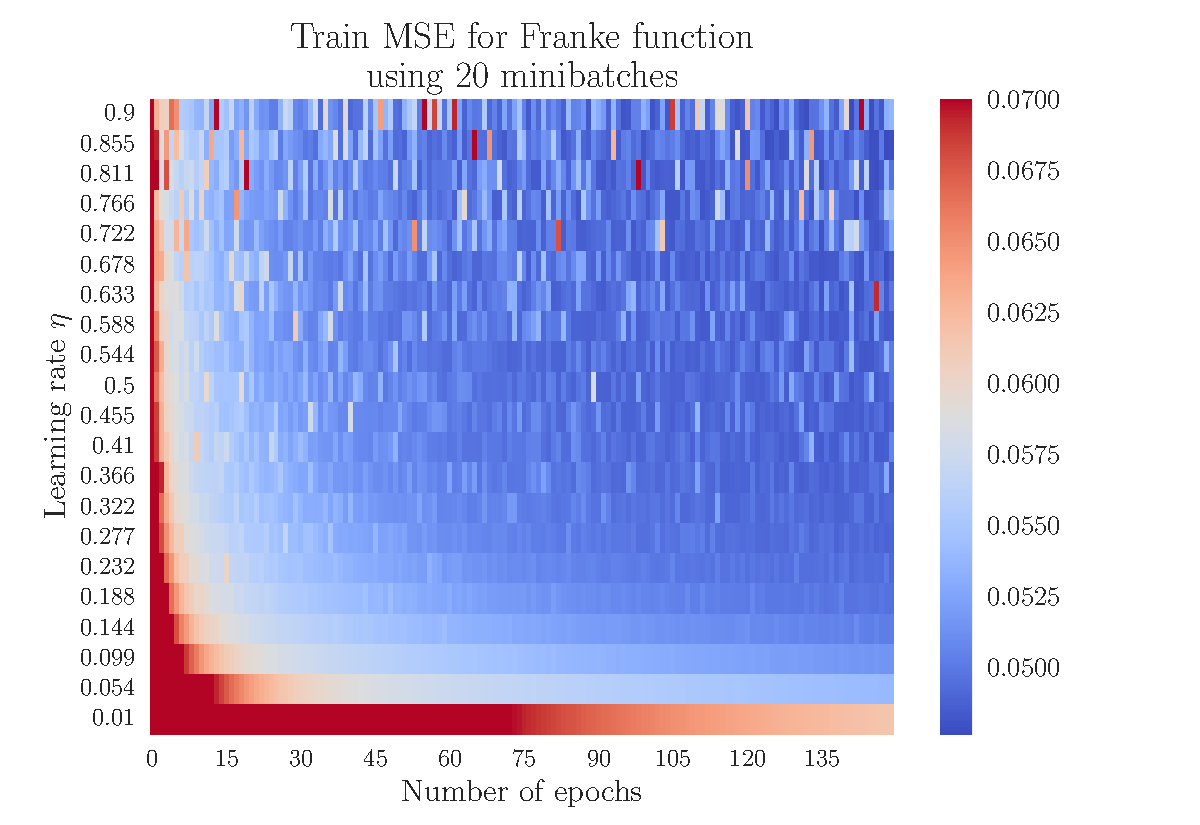
\includegraphics[width=\linewidth]{SGD_Franke/reg_Franke__epochs_eta__Train_MSE__overfit_489047.pdf}
	\endminipage
	\minipage{0.49\textwidth}
	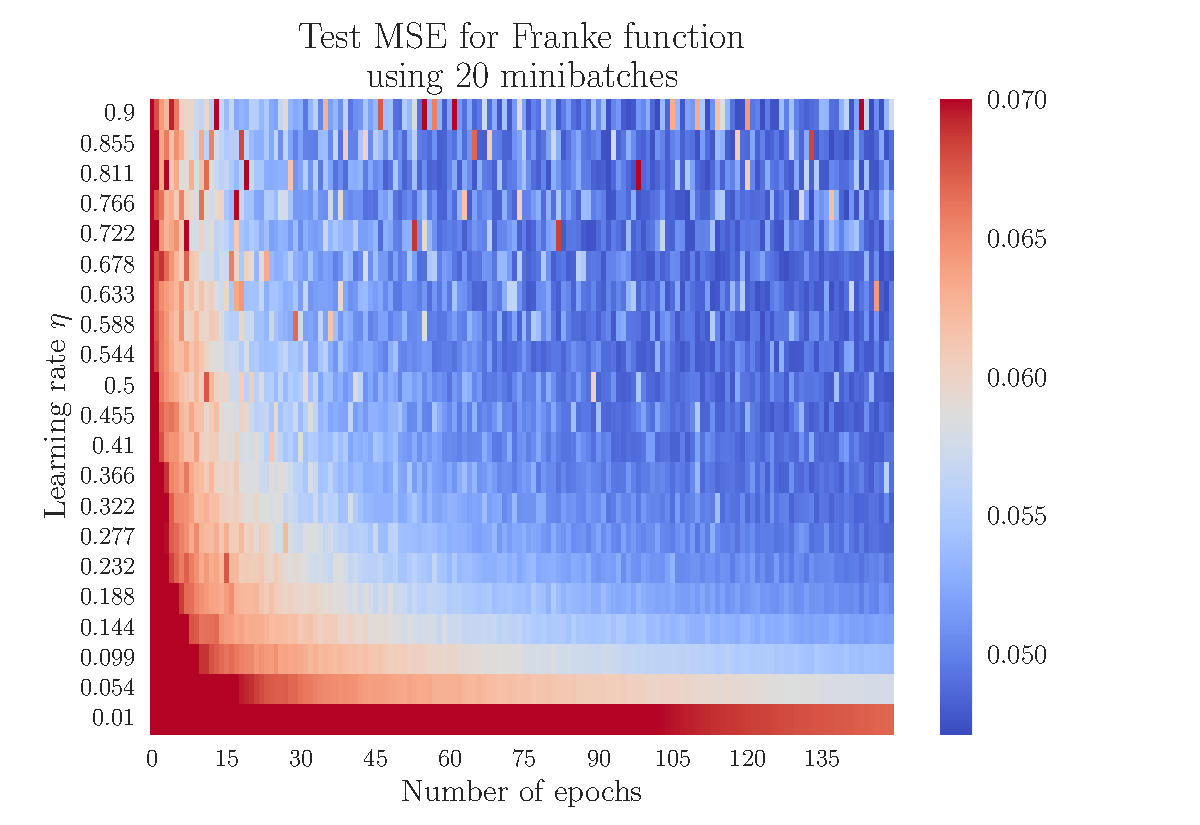
\includegraphics[width=\linewidth]{SGD_Franke/reg_Franke__epochs_eta__Test_MSE__overfit_395885.pdf}
	\endminipage
	\caption{SGD}
	\label{fig:SGD_Franke_epochs_eta_overfit}
\end{figure}

In figure \ref{fig:SGD_Franke_epochs_eta_overfit} we see that the test MSE converges faster for increased values of $\eta$ as expected. For $\eta=0.01$ we get an MSE barely below $0.07$ after $N_e=150$, as the gradient steps are too small. When $\eta$ exceeds $0.5$ we get abrubt increments of the test MSE after certain epochs. These learning rates are too high, as a gradient step goes beyond the actual minima. For $\eta=0.9$ this effect is apparent, with large fluctuations of the MSE over certain epochs. We emphasize that the bright red lines present could represent MSE values far above $0.07$.

We proceed by plotting the test MSE for $\eta\in[0.01,\,0.5]$, shown in figure \ref{fig:SGD_Franke_epochs_eta}, where we set the maximum MSE to $0.07$ once again. We clearly see how the increased learning rate yields a faster converging result, but at the expense of the MSE stability, which we can see from clear fluctuations for $\eta=0.5$. When our prediction approaches the desired model, the gradients are relatively small, such that high learning rates overshoots potential minima that we're seeking.

For studying the MSE for different number of minibatches and different momentum parameters, $\gamma$, we will choose $\eta=0.25$. In figure \ref{fig:SGD_Franke_epochs_eta}, we see that $\eta=0.25$ yields fairly quick convergence of the MSE without significant variations. Learning rates higher than this appears to be too high, while the ones below it appears to be small enough that minima of the cost function are rarely overshot. $\eta=0.25$ appears therefore to be a boundary between slow convergence and minima overshooting, and when testing other parameters we are more likely to encapsule both cases at once.

\begin{figure}[h!]
	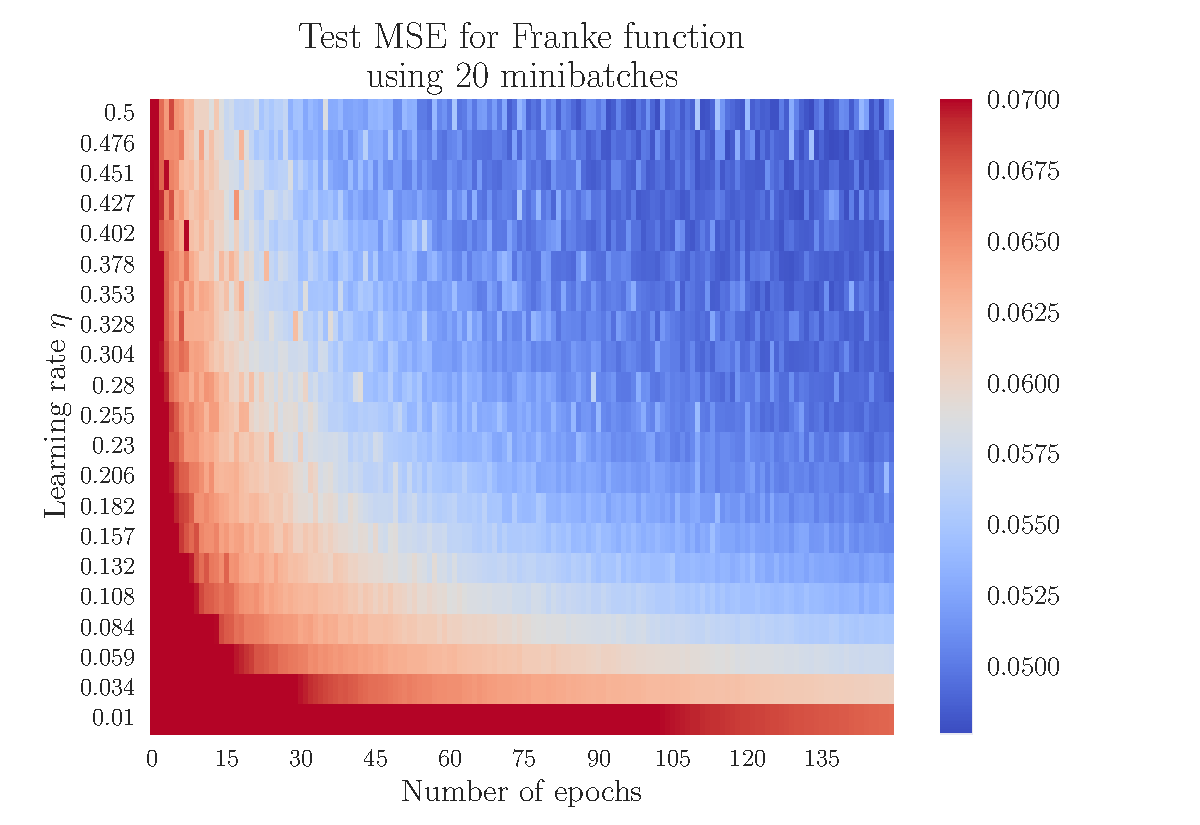
\includegraphics[width=0.9\linewidth]{SGD_Franke/reg_Franke__epochs_eta__Test_MSE__262224.pdf}
	\caption{SGD MSE eta}
	\label{fig:SGD_Franke_epochs_eta}
\end{figure}

The MSE as a function of epochs for different number of minibatches is shown in figure \ref{fig:SGD_Franke_epochs_minibatches}. The figure shows the MSE for the train and test data in the left and right panel, respectively. We use $\mathrm{MSE}_\mathrm{max}=0.07$ once again. \sn{Burde vi fjerne train MSE?}

\begin{figure}[h!]
	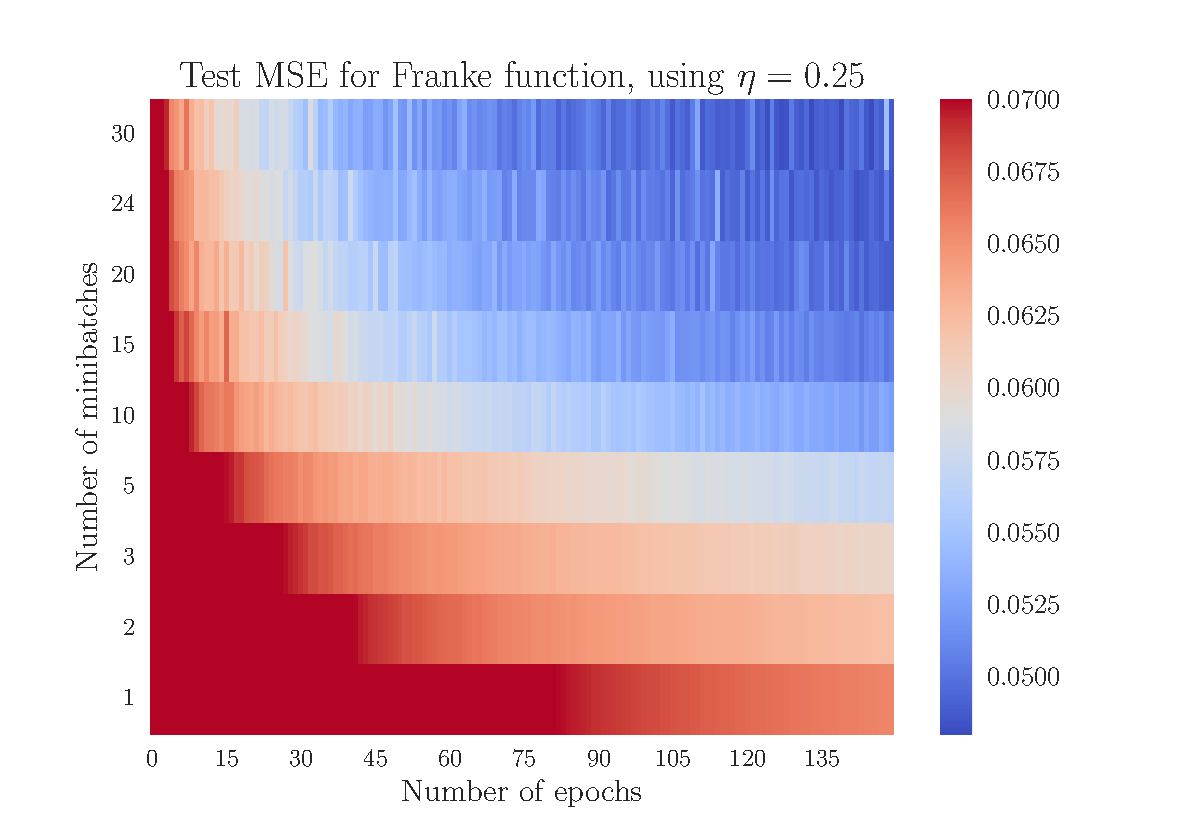
\includegraphics[width=0.9\linewidth]{SGD_Franke/reg_Franke__epochs_minibatches__Test_MSE__440533.pdf}
	\caption{SGD MSE minibatches}
	\label{fig:SGD_Franke_epochs_minibatches}
\end{figure}

Figure \ref{fig:SGD_Franke_epochs_minibatches} shows an expected behaviour of the MSE. By not using enough minibatches we are unable to get an MSE below $0.06$ after $N_e=150$, which is most likely due to the fact that we're stuck in local minima and not the global ones. When we use $N_B=30$ we get a quickly converging MSE with a low minimum value, but there appears to some fluctuations \sn{hvorfor? Er usikker på dette}.

We plot the test MSE after $N_e=150$ with different regularization parameters, shown in the left and right panel of figure \ref{fig:SGD_Franke_lambda_eta}. Using the same $\eta$ interval as before and $\lambda\leq1$ we do not set an upper limit, as we are interested in the general impact of the $\lambda$ values, and not seeking nuances of the lowest values as before. From figure \ref{fig:SGD_Franke_lambda_eta} we get a result coinciding with the ones obtained from previous linear regression study, where optimal fitting appears to be achieved as $\lambda\to0$, essentially telling us that it it redundant when fitting the Franke function.

\begin{figure}[h!]
	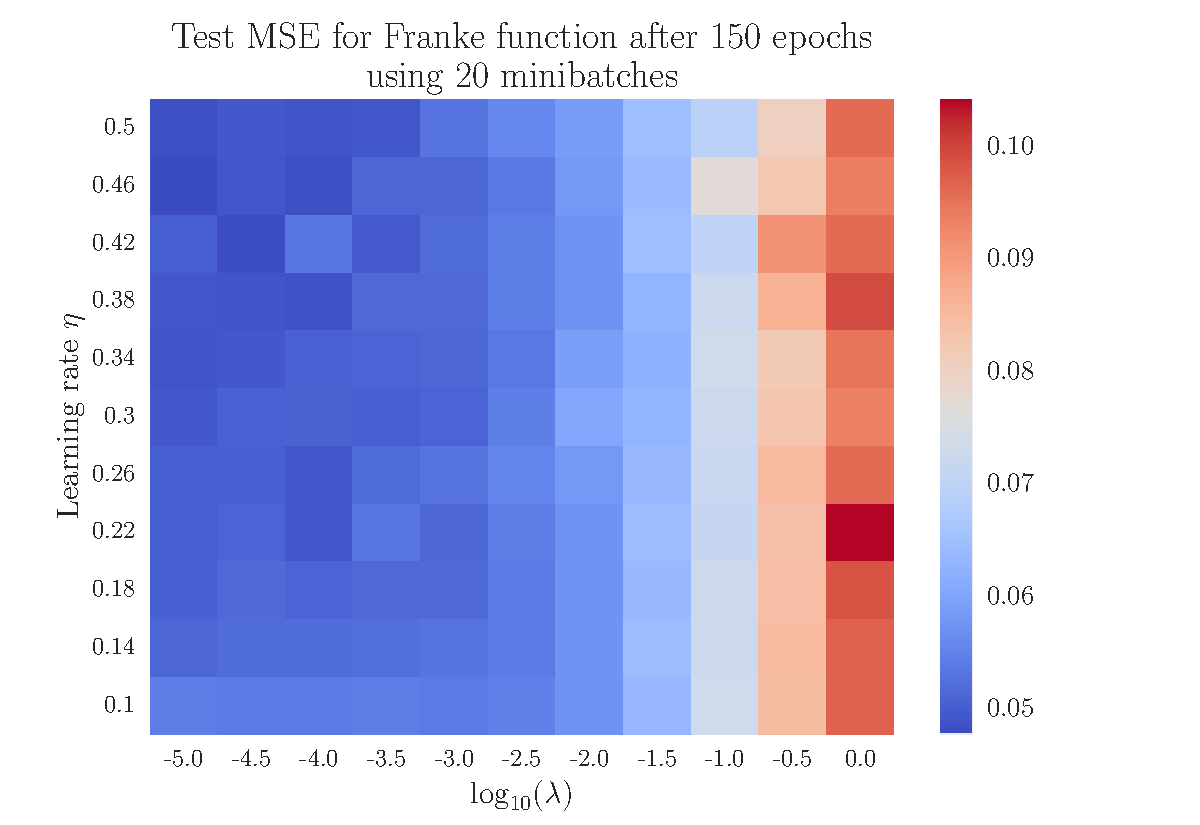
\includegraphics[width=0.9\linewidth]{SGD_Franke/reg_Franke__lambda_eta__Test_MSE__764274.pdf}
	\caption{SGD lambda}
	\label{fig:SGD_Franke_lambda_eta}
\end{figure}


Figure \ref{fig:SGD_Franke_epochs_gamma} shows the resulting MSE values for the test data with different momentum parameters as a function of $N_e\in[0,\,150]$. For this plot we have chosen an upper limit of $0.06$ for the MSE,

\begin{figure}[h!]
	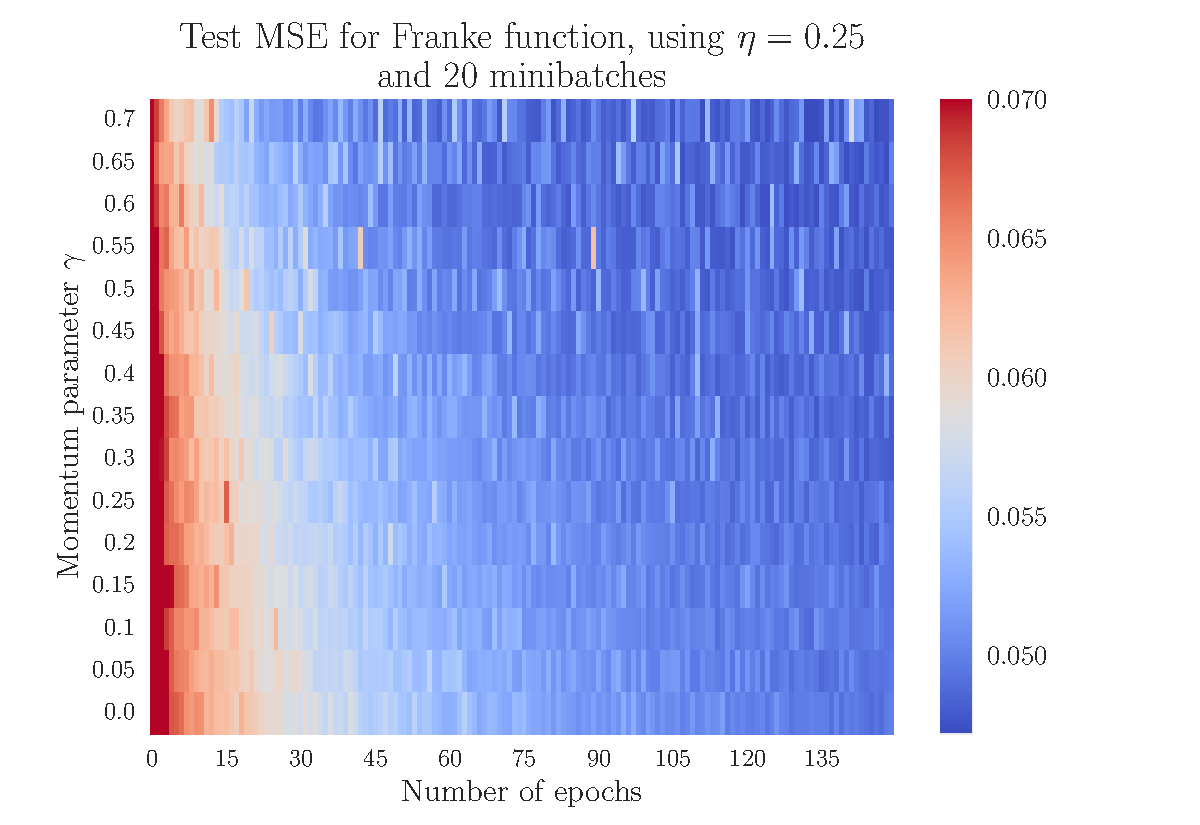
\includegraphics[width=0.9\linewidth]{SGD_Franke/reg_Franke__epochs_gamma__Test_MSE__239373.pdf}
	\caption{SGD}
	\label{fig:SGD_Franke_epochs_gamma}
\end{figure}

\begin{figure}[h!]  % kommentert ut pga manglende fil. 
	% 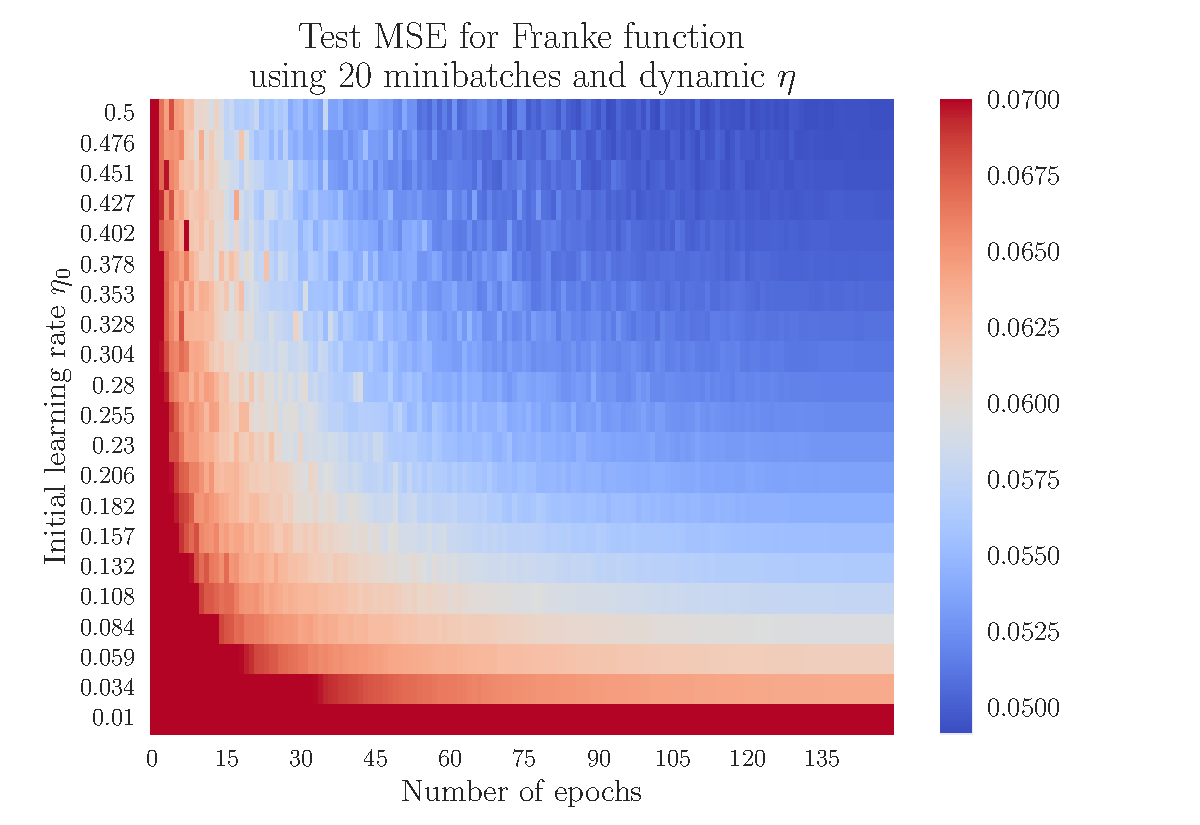
\includegraphics[width=0.9\linewidth]{SGD_Franke/reg_Franke__epochs_dynamic_eta__Test_MSE__676588.pdf}
	\includegraphics[width=0.9\linewidth]{404.png}
	\caption{SGD}
	\label{fig:SGD_Franke_epochs_dynamic_eta} 
\end{figure}


\subsubsection{Feed Forward Neural Network}
We plot

\begin{figure}[h!]
	\minipage{0.49\textwidth}
	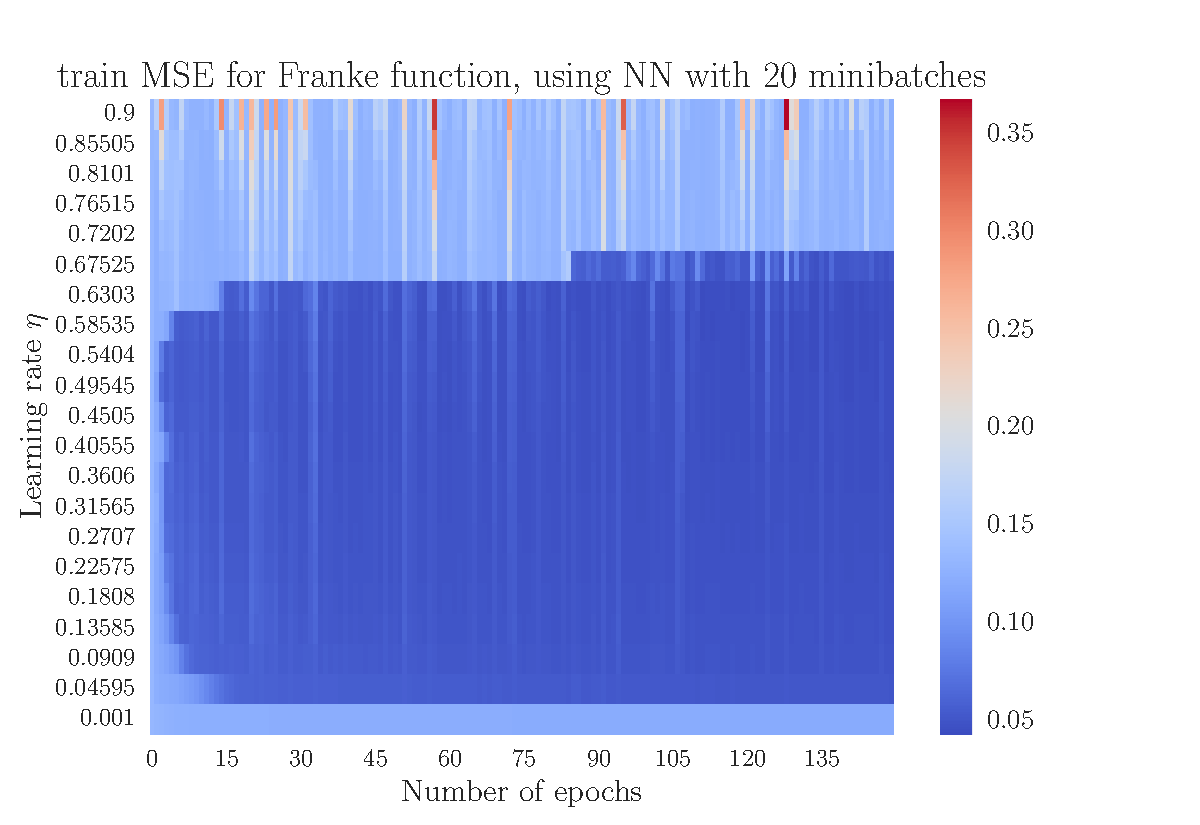
\includegraphics[width=\linewidth]{NN_Franke/NN_Franke__epochs_eta__train_MSE__569887.pdf}
	\endminipage
	\minipage{0.49\textwidth}
	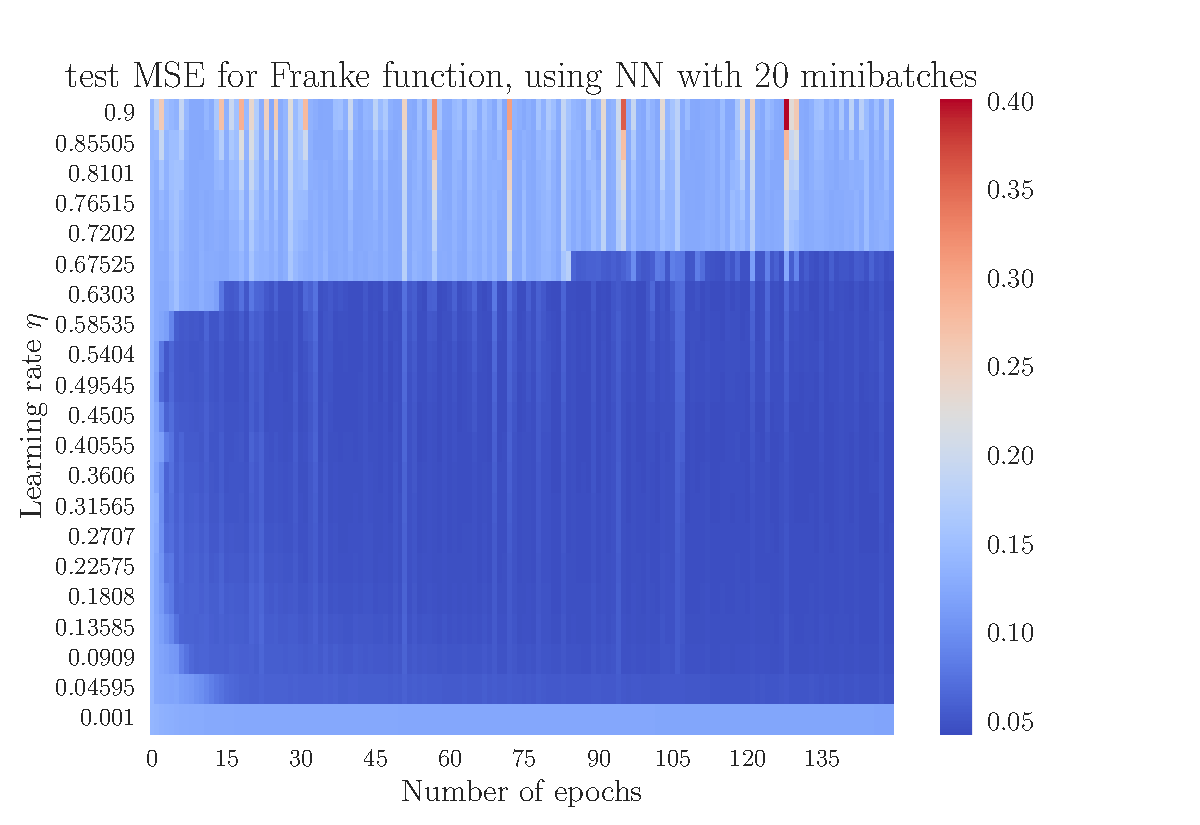
\includegraphics[width=\linewidth]{NN_Franke/NN_Franke__epochs_eta__test_MSE__271070.pdf}
	\endminipage
	\caption{NN}
	\label{fig:NN_Franke_epochs_eta_MSE}
\end{figure}


\begin{figure}[h!]
	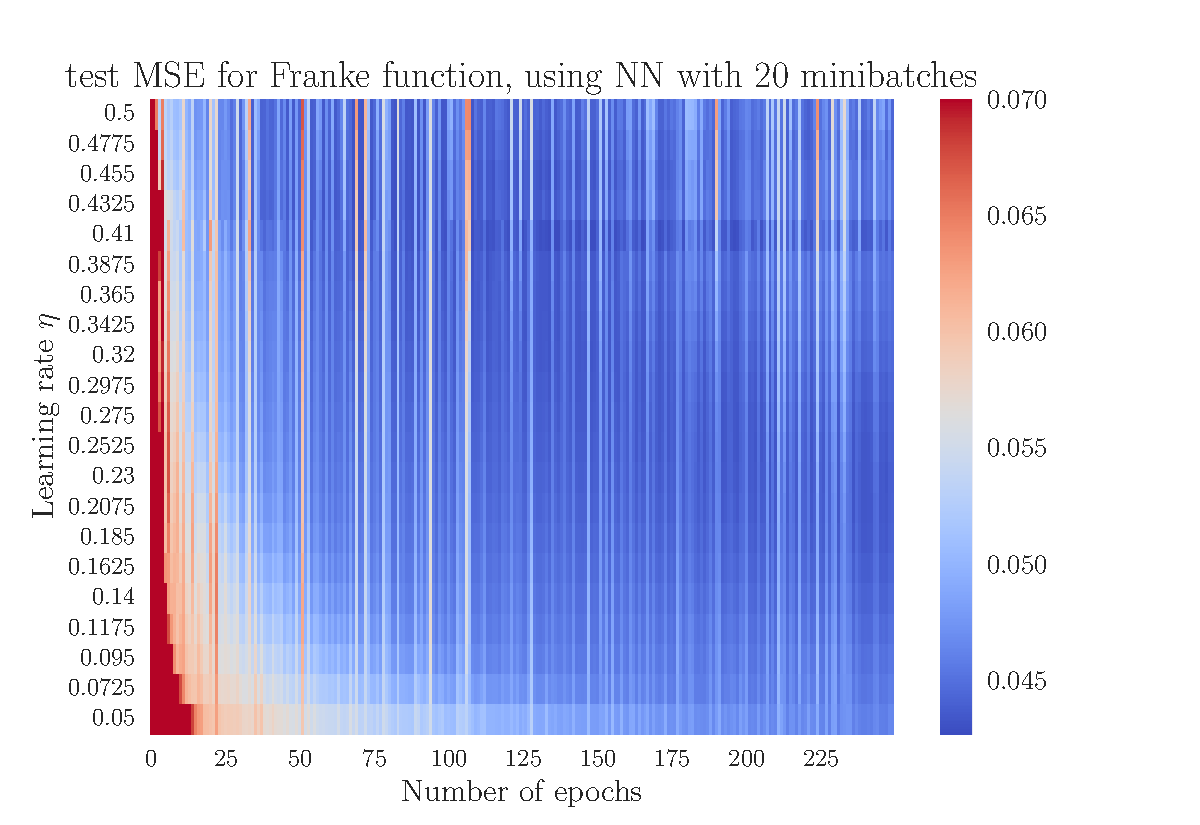
\includegraphics[width=\linewidth]{NN_Franke/NN_Franke__epochs_eta__test_MSE__582234.pdf}
	\caption{NN}
	\label{fig:NN_Franke_epochs_eta_MSE_limited}
\end{figure}

\begin{figure}[h!]
	\minipage{0.49\textwidth}
	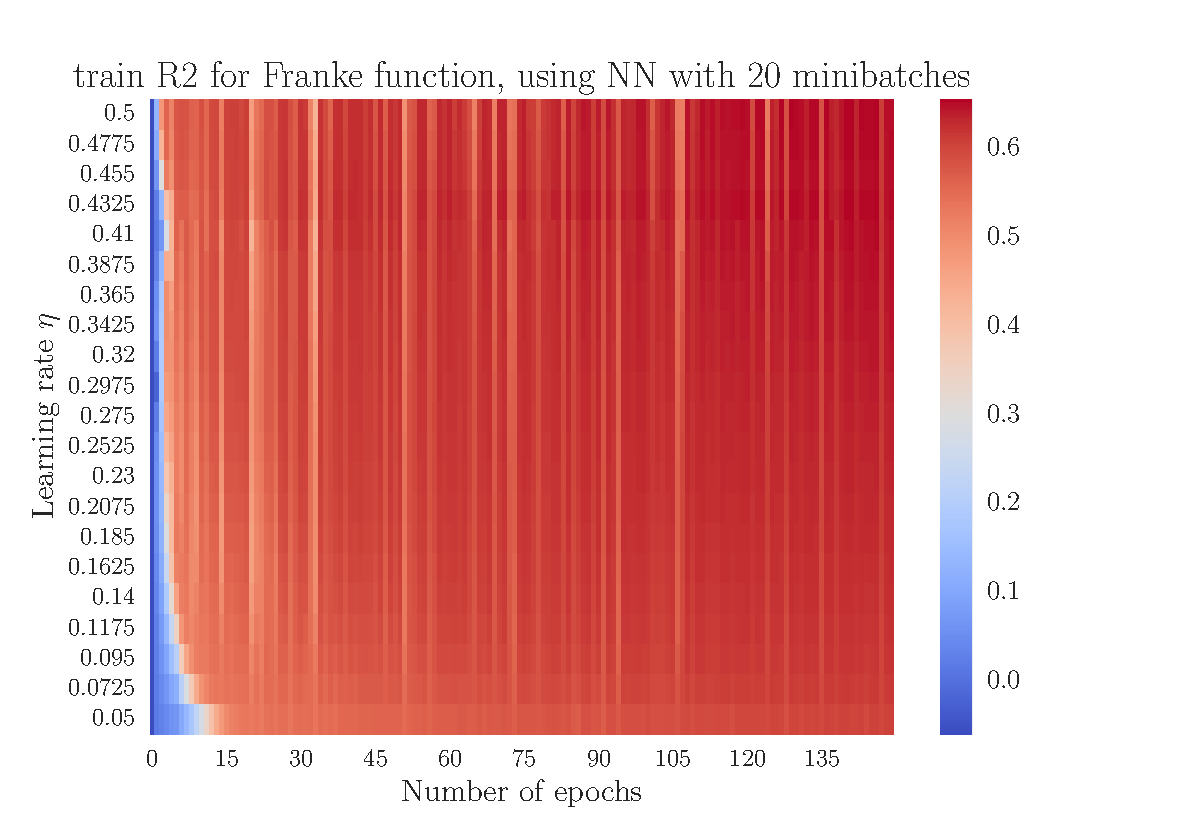
\includegraphics[width=\linewidth]{NN_Franke/NN_Franke__epochs_eta__train_R2__738371.pdf}
	\endminipage
	\minipage{0.49\textwidth}
	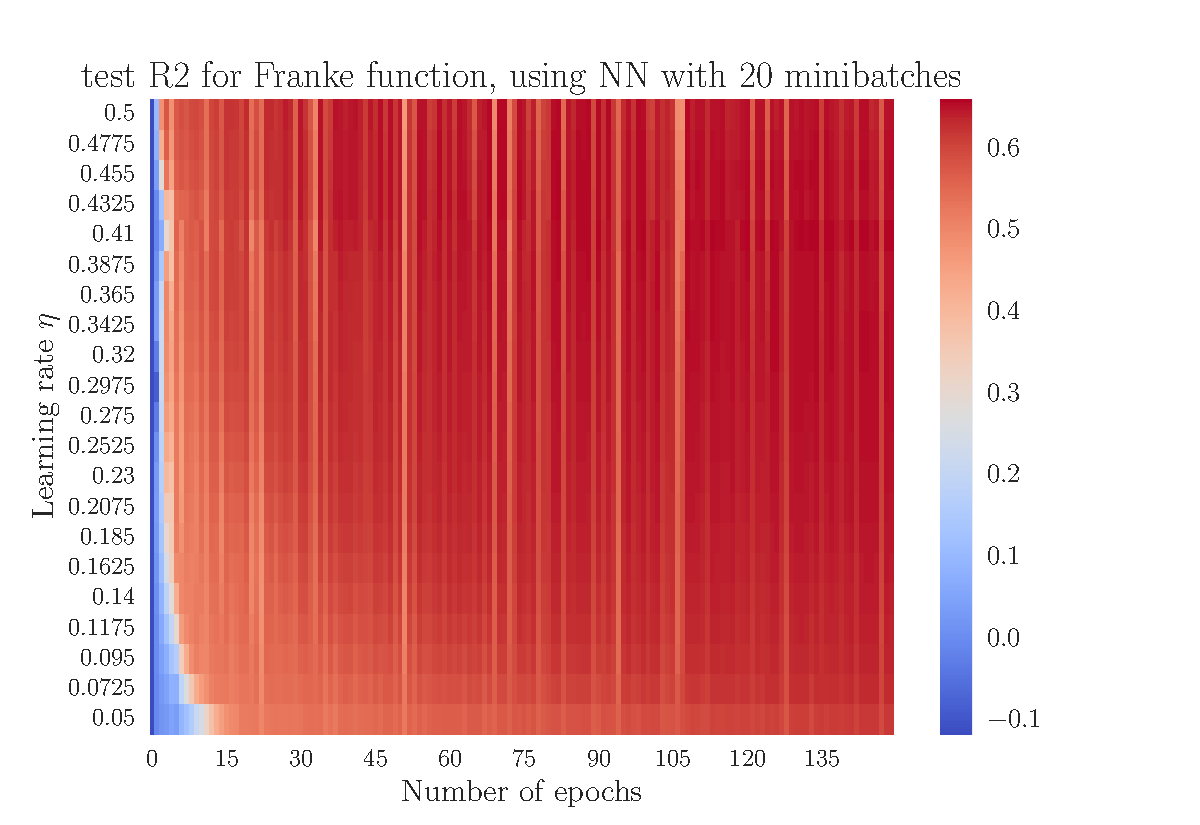
\includegraphics[width=\linewidth]{NN_Franke/NN_Franke__epochs_eta__test_R2__296747.pdf}
	\endminipage
	\caption{NN}
	\label{fig:NN_Franke_epochs_eta_R2}
\end{figure}

\begin{figure}[h!]
	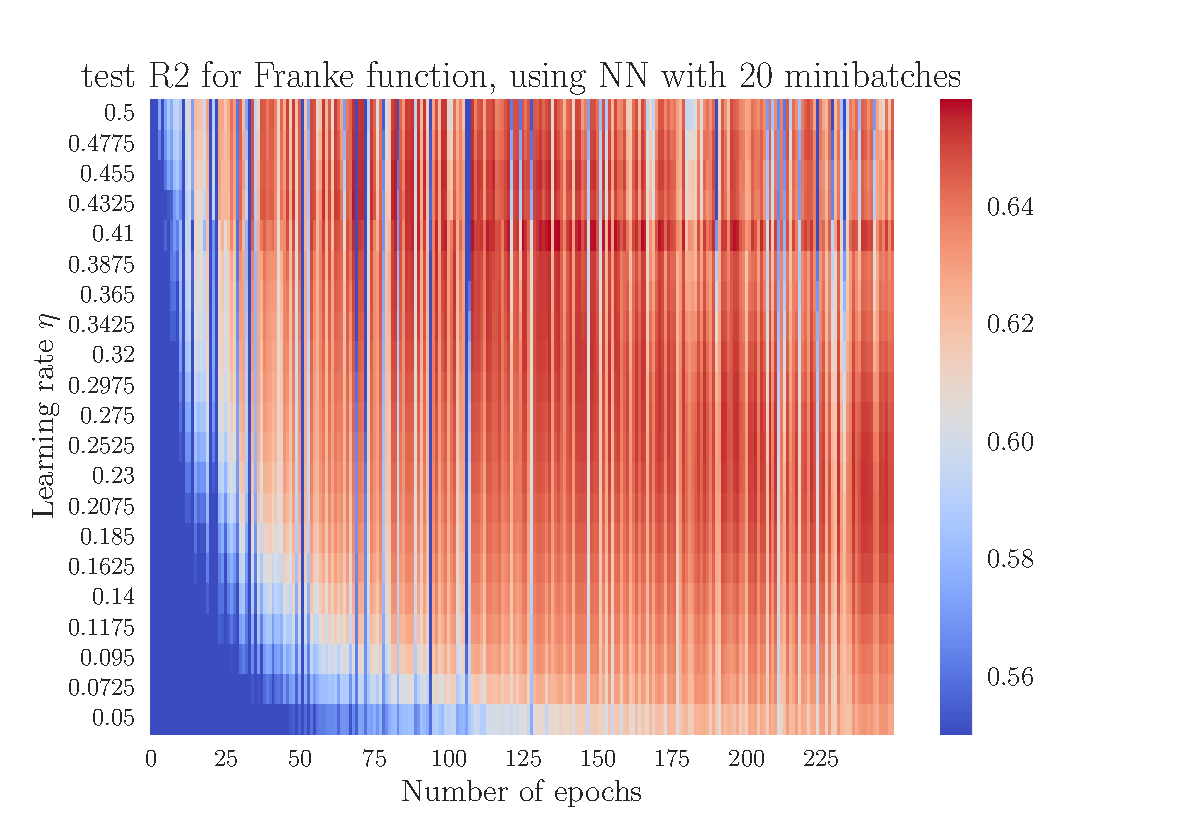
\includegraphics[width=\linewidth]{NN_Franke/NN_Franke__epochs_eta__test_R2__190748.pdf}
	\caption{NN}
	\label{fig:NN_Franke_epochs_eta_R2_limited}
\end{figure}

\begin{figure}[h!]
	\minipage{0.49\textwidth}
	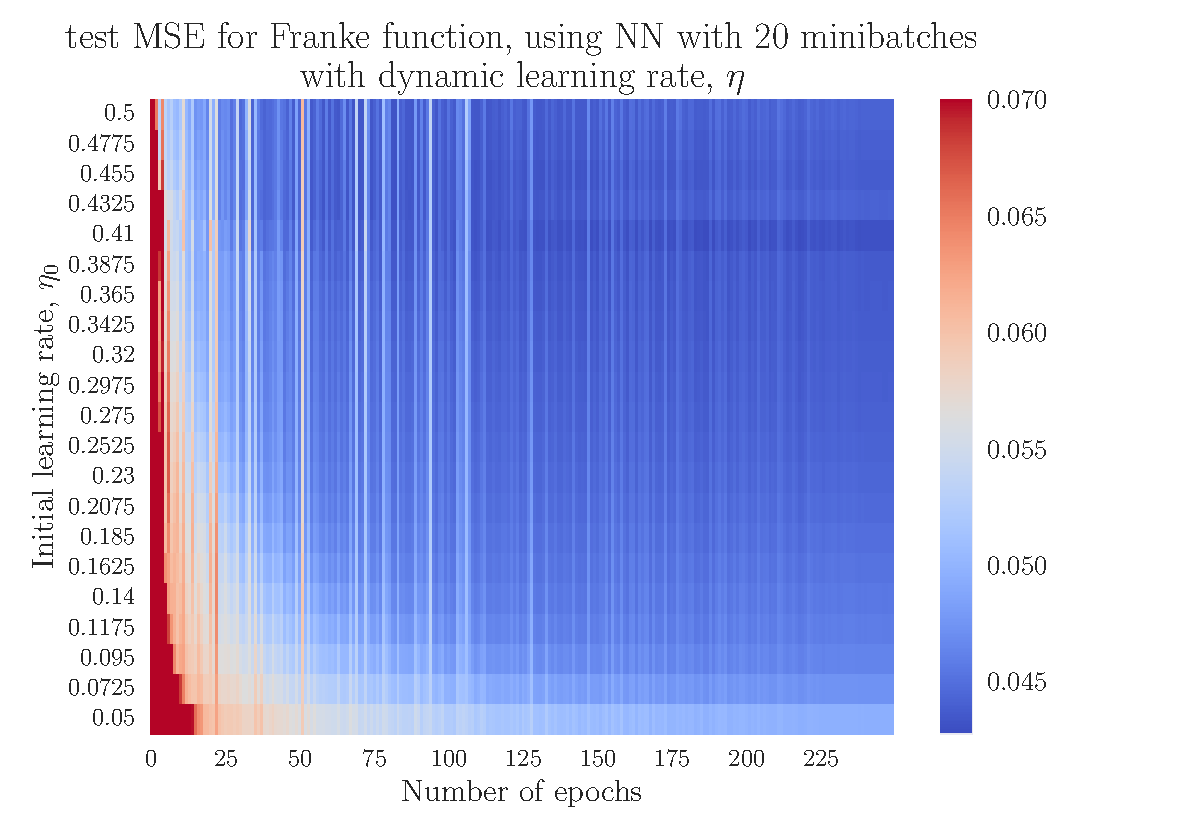
\includegraphics[width=\linewidth]{NN_Franke/NN_Franke__epochs_dynamic_eta__test_MSE__489375.pdf}
	\endminipage
	\minipage{0.49\textwidth}
	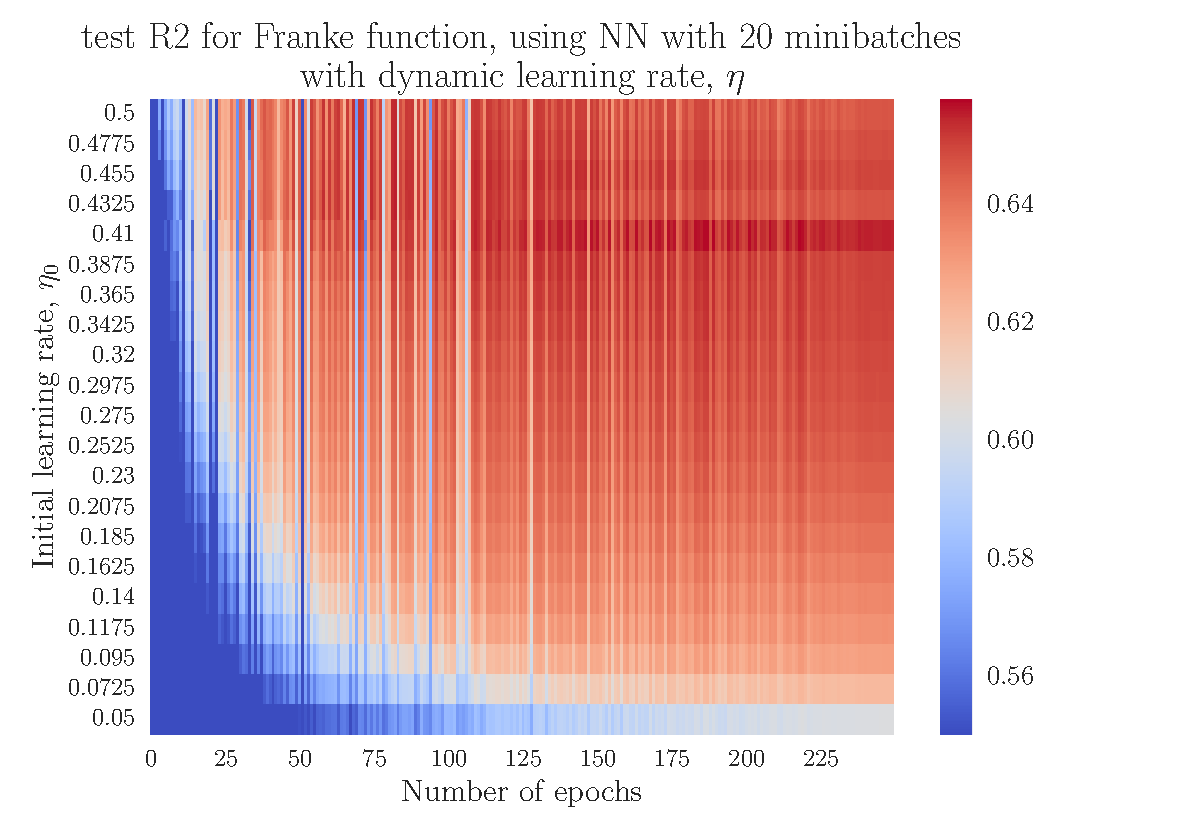
\includegraphics[width=\linewidth]{NN_Franke/NN_Franke__epochs_dynamic_eta__test_R2__289368.pdf}
	\endminipage
	\caption{NN}
	\label{fig:NN_Franke_epochs_dynamic_eta}
\end{figure}

\begin{figure}[h!]
	\minipage{0.49\textwidth}
	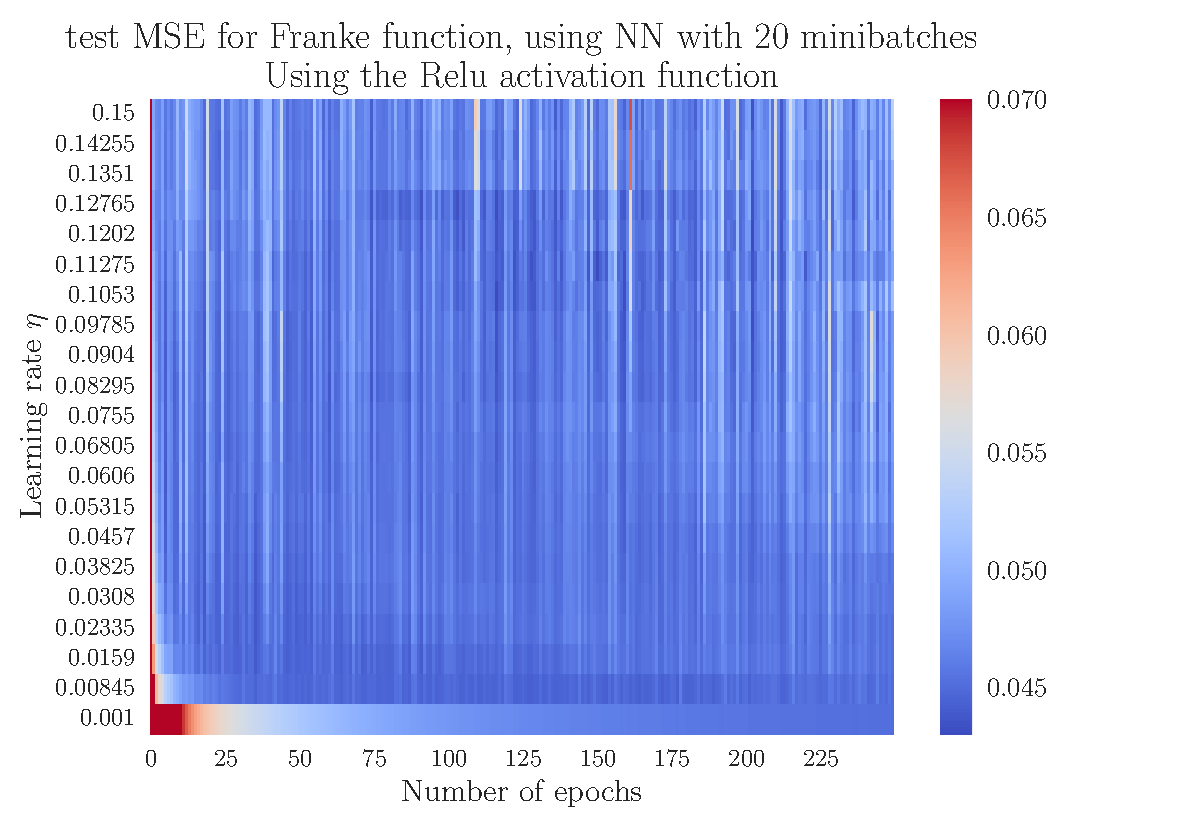
\includegraphics[width=\linewidth]{NN_Franke/NN_Franke__epochs_eta__test_MSE__relu__733938.pdf}
	\endminipage
	\minipage{0.49\textwidth}
	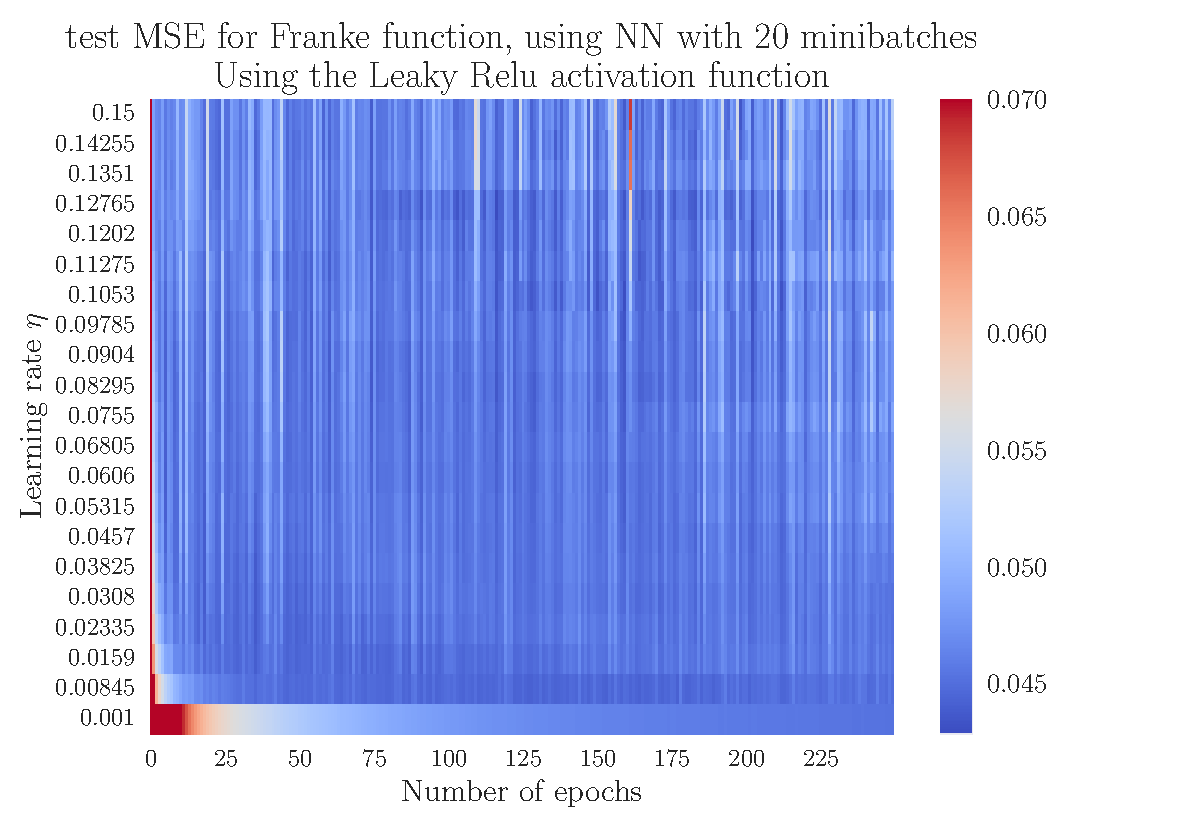
\includegraphics[width=\linewidth]{NN_Franke/NN_Franke__epochs_eta__test_MSE__leaky_relu__501404.pdf}
	\endminipage
	\caption{MSE Relu and Leaky Relu}
	\label{fig:NN_Franke_epochs_eta_MSE_relu_leaky}
\end{figure}

\begin{figure}[h!]
	\minipage{0.49\textwidth}
	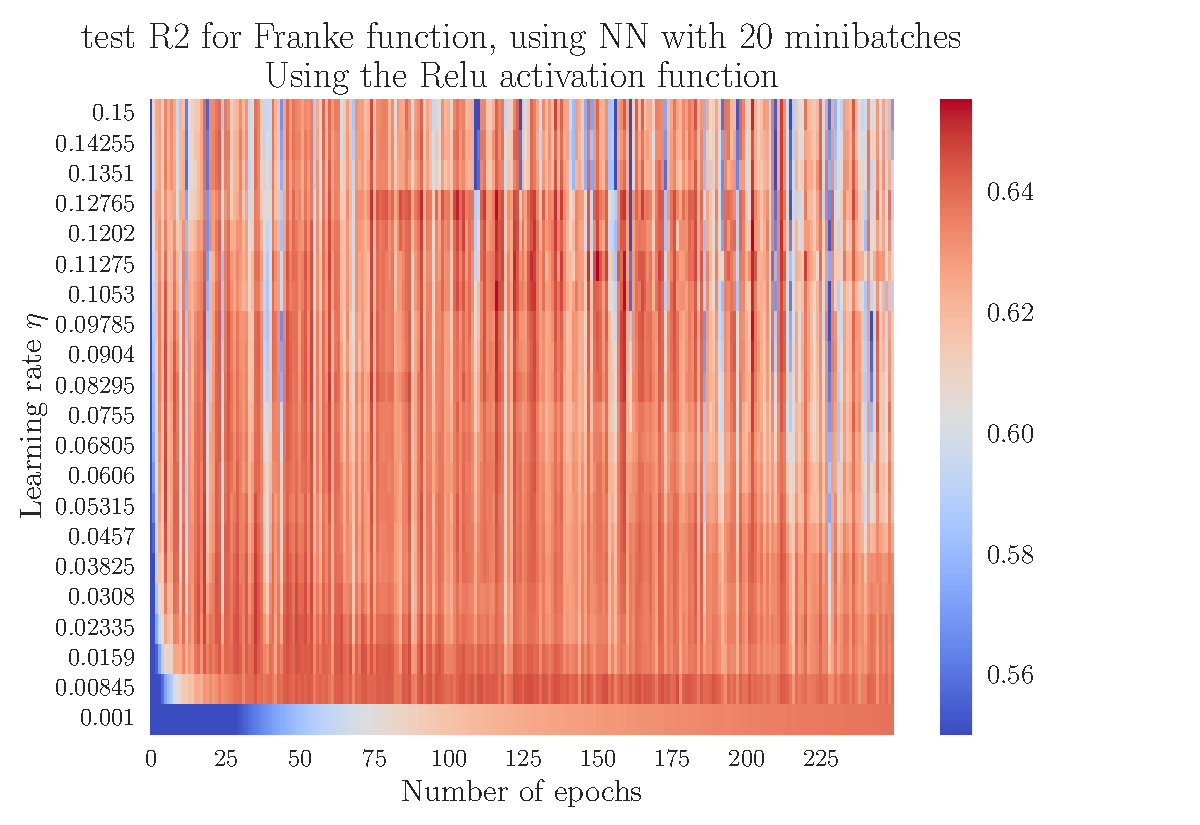
\includegraphics[width=\linewidth]{NN_Franke/NN_Franke__epochs_eta__test_R2__relu__235205.pdf}
	\endminipage
	\minipage{0.49\textwidth}
	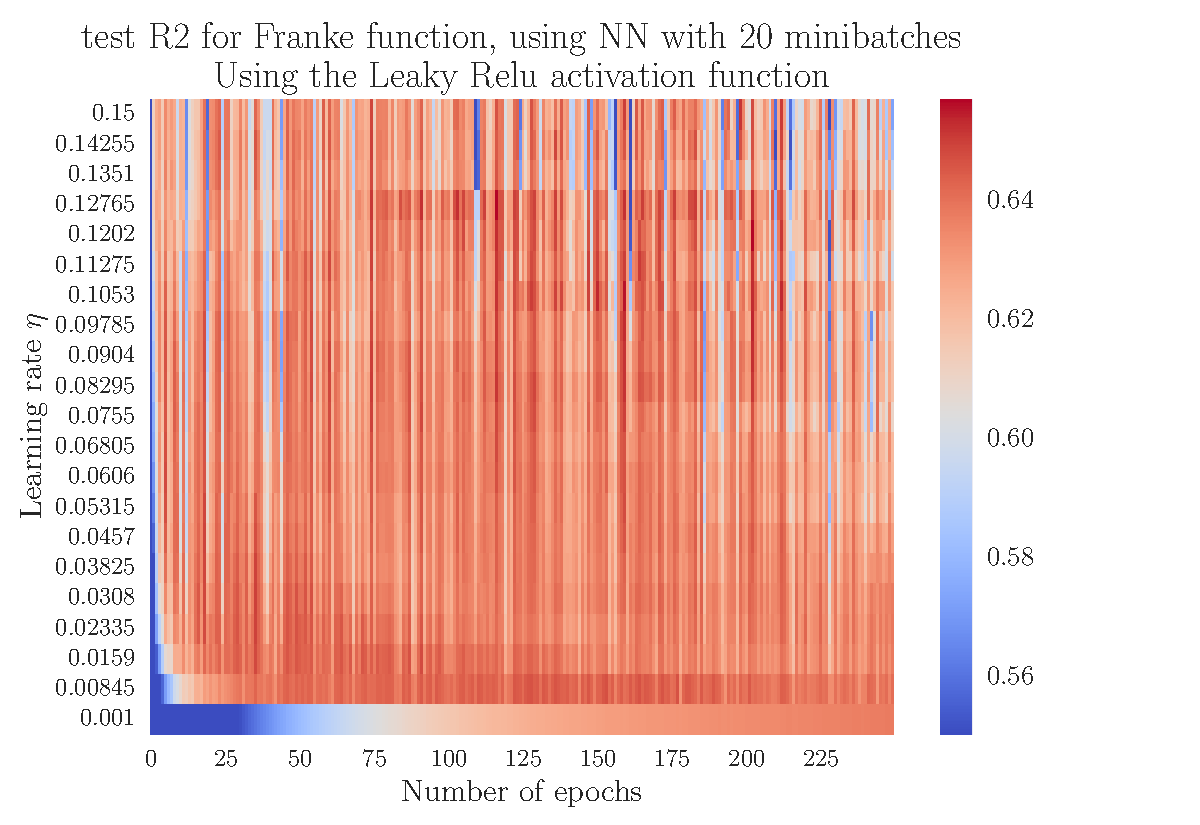
\includegraphics[width=\linewidth]{NN_Franke/NN_Franke__epochs_eta__test_R2__leaky_relu__958829.pdf}
	\endminipage
	\caption{R2 Relu and Leaky Relu}
	\label{fig:NN_Franke_epochs_eta_R2_relu_leaky}
\end{figure}

\subsection{Wisconsin Breast Cancer Data}
\subsubsection{Feed Forward Neural Network}
\subsubsection{Logistic Regression}

In figure \ref{fig:logreg_eta_epoch} we plot the accuracy score as a function of epochs, for different learning rates $\eta$ and $L_2$ parameter set to $\lambda = 0$. The top plot is for the train data, and bottom for test data. We notice, as expected, that for a low enough $\eta$ we get under fitting. Especially for $\eta = 10^{-3}$
\begin{figure}[h]
	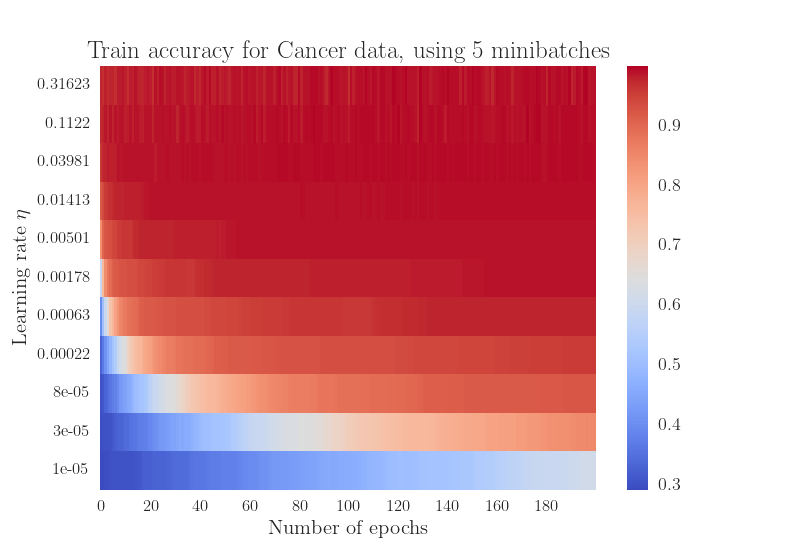
\includegraphics[width=\linewidth]{../output/plots/reg_Cancer__epochs_eta__Train_accuracy__705107.png}
	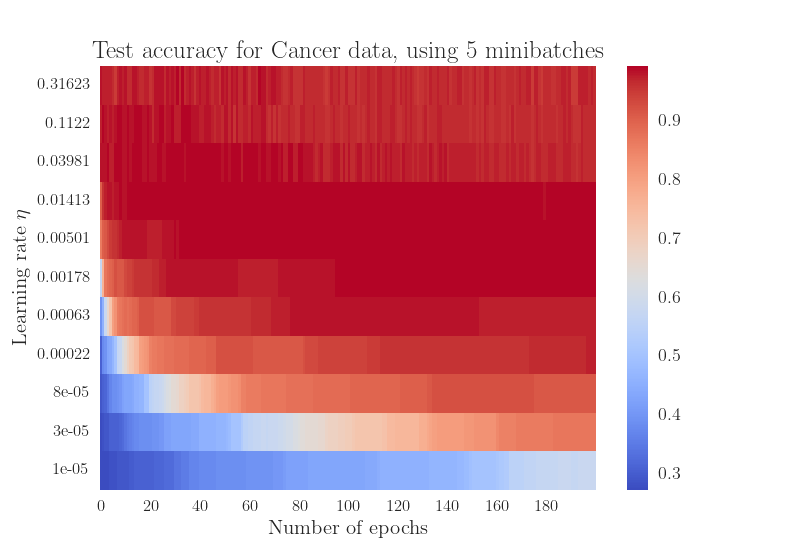
\includegraphics[width=\linewidth]{../output/plots/reg_Cancer__epochs_eta__Test_accuracy__924831.png}
	\caption{These two figures illustrates how the accuracy score evolves as a function of epochs ($x$-axis) and learning rate $\eta$ ($y$-axis). An accuracy score of one corresponds to 100\% correct classifications.}\label{fig:logreg_eta_epoch}
\end{figure}
\begin{figure}[h]
	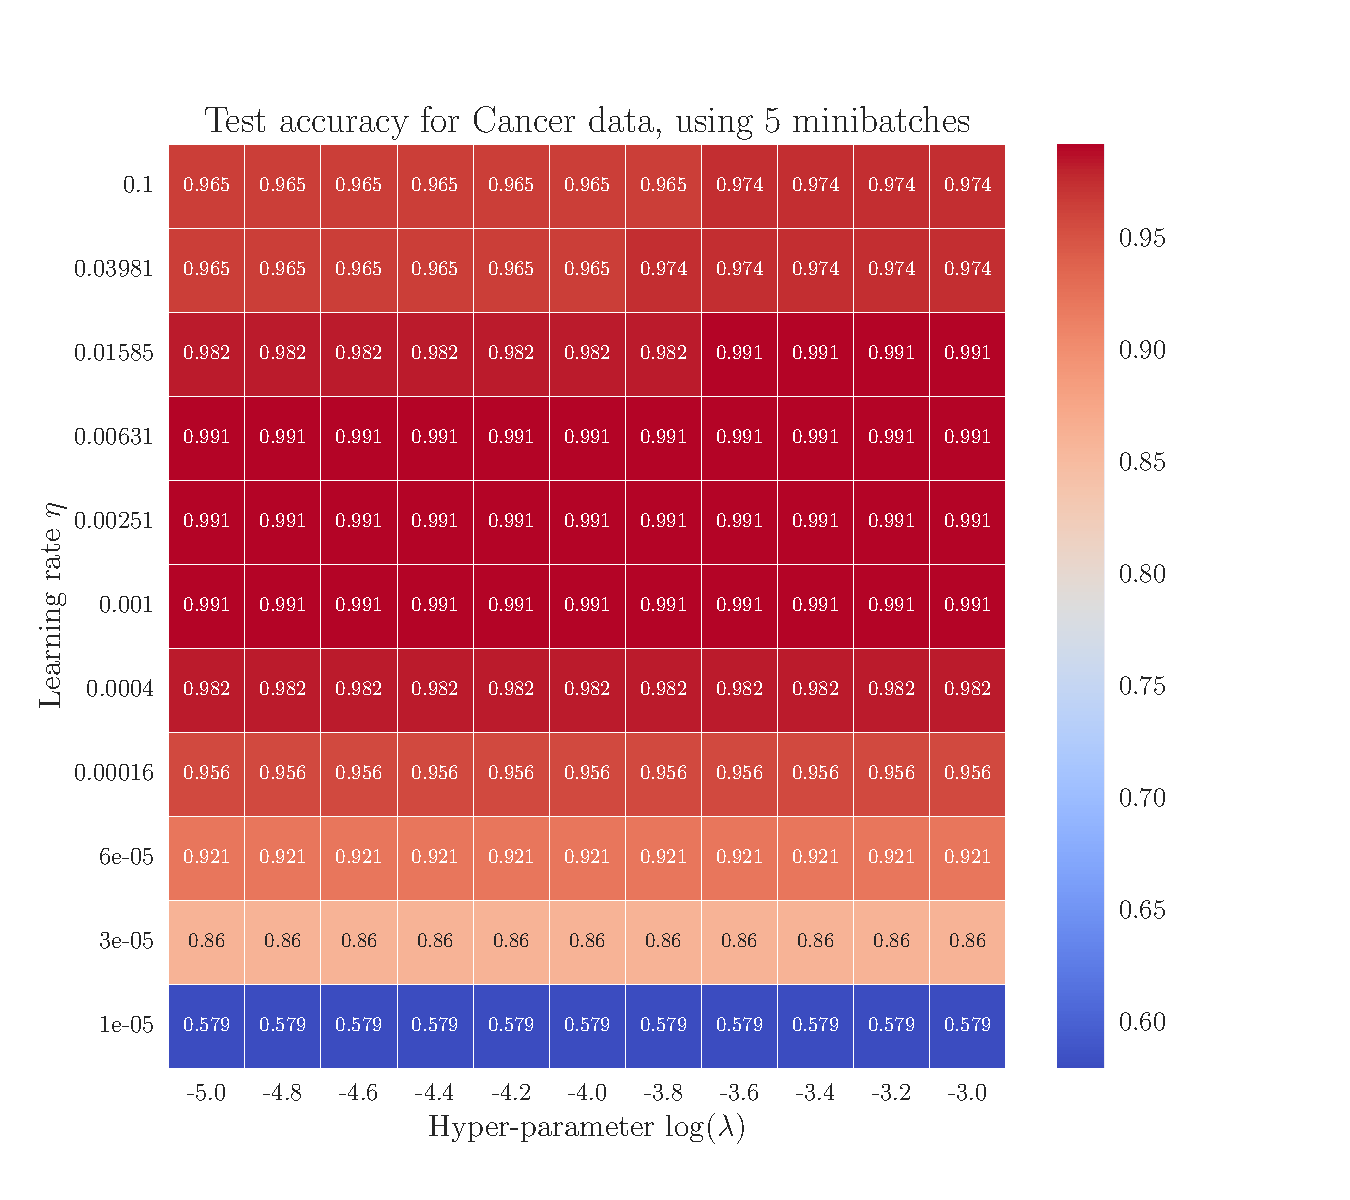
\includegraphics[width=\linewidth]{../output/plots/reg_Cancer__lambda_eta__Test_accuracy__860729.pdf}
	\caption{Here we have plotted the accuracy for the test data, as a function of both learning rate $\eta$ ($y$-axis) and logarithm of hyper parameter $\lambda$ ($x$-axis). An accuracy score of one corresponds to 100\% correct classification.}\label{fig:logreg_eta_lambda}
\end{figure}



\section{Discussion}


LOGISTIC REGRESSION:

momentum

different output functions

learning schedule

correlation

hvor sikkert er nettverket?
\section{Conclusion}


\bibliographystyle{plain}
\bibliography{refs}
\end{document}

